\documentclass[dscexam, EN]{ufabcFHZh}
%% =============================
%%      IMPORTANTE
%% ESTE ARQUIVO DEVE ESTAR SALVO COMO
%%      UTF - 8
%% =============================

% ----------------------------------------------------------
% Este capítulo é parte integrante do arquivo mestre
% Relatorio_TCC_Mestrado_Base_VERSÃO_SUBVERSÃO
% ----------------------------------------------------------

%==== Novos comandos para escrever nomes pré-formatados
%---
\newcommand{\ufabcFHZ}
{\textbf{\textit{ufabcFHZh.cls}}}
%---
\newcommand{\abntFHZ}
{\textbf{\textit{abntFHZ5.bst}}}
%---
\newcommand{\Fonte}[1]
{{\footnotesize Fonte: #1.}}
%---
\newcommand{\Oautor}
{O autor}
%---
\newcommand{\matlab}
%{Matlab$^\circledR$}
{Matlab\textsuperscript{\textregistered}}
%---
\newcommand{\simulink}
{Simulink\textsuperscript{\textregistered}}
%---
\newcommand{\matlabsimulink}
{Matlab/Simulink\textsuperscript{\textregistered}}
%---
\newcommand{\arduino}
{Arduino\textsuperscript{\textregistered}}
%---
\newcommand{\arduinomega}
{Arduino\textsuperscript{\textregistered} Mega}

%---
\newcommand{\DINAMA}
{\textit{DINAMA}}
%---
\newcommand{\excel}
{Excel\textsuperscript{\textregistered}}
%---
\newcommand{\projetoDaniel}
{\textit{Projeto Daniel}}
%---
\newcommand{\notimpossiblenow}
{\textit{Not Impossible\textsuperscript{Now}}}
%---
\newcommand{\caltech}
{\textit{Caltech}}
%====

% ----------------------------------------- 
% Formas de uso de condicional ifthenelse / toogle para selecionar cores de links
% -----------------------------------------
% http://alvinalexander.com/blog/post/latex/two-simple-examples-using-latex-ifthen-package
% http://tex.stackexchange.com/questions/5894/latex-conditional-expression
% -----------------------------------------
\usepackage{etoolbox} 		% Permite o uso de \newtoggle para criar desvios de fluxo
\usepackage{pdfpages}
%---
\newtoggle{LinksComCores} 	% Opção para selecionar entre links sem cores ou coloridos
% ===
% -----------------------------------------

% ----------------------------------------------------------
% Fim Arquivo
% \usepackage[alf, abnt-emphasize=bf, abnt-thesis-year=both, abnt-repeated-author-omit=no, abnt-last-names=abnt, abnt-etal-cite=3, abnt-etal-list=3, abnt-etal-text=it, abnt-and-type=e, abnt-doi=doi, abnt-url-package=none, abnt-verbatim-entry=no]{abntex2cite}

% Set same dot spacing for list of figures/tables and list of symbols 
%\usepackage{tocbasic}

%\newcommand\Dotfill{\cftdotfill{\cftsecdotsep}}
%   \renewcommand{\cftchapleader}{\cftdotfill{\cftsecdotsep}}


\newcommand{\plotdrs}[4]{ 
\begin{figure}[t]
    \centering
    \begin{subfigure}{0.32\textwidth}
        \centering
        % include second image
        \includegraphics[width=\linewidth]{Figuras/drs/#1/doe_200/drs_#2_all_#3_surface.pdf}  
        \caption{Small dataset.}
        \label{fig:drs_#2_#3_200}
    \end{subfigure}
    \begin{subfigure}{0.32\textwidth}
        \centering
        % include second image
        \includegraphics[width=\linewidth]{Figuras/drs/#1/doe_500/drs_#2_all_#3_surface.pdf}  
        \caption{Medium dataset.}
        \label{fig:drs_#2_#3_500}
    \end{subfigure}
    \begin{subfigure}{0.32\textwidth}
        \centering
        \includegraphics[width=\linewidth]{Figuras/drs/#1/doe_1000/drs_#2_all_#3_surface.pdf}  
        \caption{Large dataset}
        \label{fig:drs_#2_#3_1000}
    \end{subfigure}
    \caption{#4}
    \label{fig:drs_#2_#3}
\end{figure}
}

\newcommand{\plothpoboxplot}[3]{ 
\begin{figure}[t]
    \centering
    \begin{subfigure}{0.3\textwidth}
        \centering
        % include second image
        \includegraphics[width=\linewidth]{Figuras/hpo/hpo_plots_#1_#2/hpo_nn_activation_MAPE.pdf}  
        \caption{MAPE.}
        \label{fig:hpo_MAPE_a#1_#2}
    \end{subfigure}
    \begin{subfigure}{0.3\textwidth}
        \centering
        % include second image
        \includegraphics[width=\linewidth]{Figuras/hpo/hpo_plots_#1_#2/hpo_nn_activation_NRMSE.pdf}  
        \caption{NRMSE.}
        \label{fig:hpo_NRMSE_#1_#2}
    \end{subfigure}
    \begin{subfigure}{0.3\textwidth}
        \centering
        \includegraphics[width=\linewidth]{Figuras/hpo/hpo_plots_#1_#2/hpo_nn_activation_R2.pdf}  
        \caption{R2}
        \label{fig:hpo_R2_#1_#2}
    \end{subfigure}
    \caption{#3}
    \label{fig:hpo_#1_#2}
\end{figure}
}

\newcommand{\plothpomap}[3]{
\begin{figure}[t]
    \centering
    \begin{subfigure}{0.3\textwidth}
        \centering
        % include second image
        \includegraphics[width=\linewidth]{Figuras/hpo/hpo_plots_#1_#2/neurons_layers_heat_map_MAPE.pdf}  
        \caption{MAPE.}
        \label{fig:hpo_map_MAPE_all_all}
    \end{subfigure}
    \begin{subfigure}{0.3\textwidth}
        \centering
        % include second image
        \includegraphics[width=\linewidth]{Figuras/hpo/hpo_plots_#1_#2/neurons_layers_heat_map_NRMSE.pdf}  
        \caption{NRMSE.}
        \label{fig:hpo_map_NRMSE_all_all}
    \end{subfigure}
    \begin{subfigure}{0.3\textwidth}
        \centering
        \includegraphics[width=\linewidth]{Figuras/hpo/hpo_plots_#1_#2/neurons_layers_heat_map_R2.pdf}  
        \caption{R2}
        \label{fig:hpo_map_R2_all_all}
    \end{subfigure}
    \caption{#3}
    \label{fig:hpo_map_all_all}
\end{figure}
}

\newcommand{\plothpohistogram}[3]{
\begin{figure}[t]
    \centering
    \begin{subfigure}{0.3\textwidth}
        \centering
        % include second image
        \includegraphics[width=\linewidth]{Figuras/hpo/hpo_plots_#1_#2/hpo_nn_hist_neurons_layers.pdf}  
        \caption{Histogram neurons layers.}
        \label{fig:hpo_hist_neurons_#1_#2}
    \end{subfigure}
    \begin{subfigure}{0.3\textwidth}
        \centering
        % include second image
        \includegraphics[width=\linewidth]{Figuras/hpo/hpo_plots_#1_#2/hpo_nn_activation_layers_count.pdf}  
        \caption{Histogram activation layers.}
        \label{fig:hpo_hist_activation_#1_#2}
    \end{subfigure}
    \begin{subfigure}{0.3\textwidth}
        \centering
        \includegraphics[width=\linewidth]{Figuras/hpo/hpo_plots_#1_#2/hpo_nn_activation_layers_surface.pdf}  
        \caption{Surface MAPE}
        \label{fig:hpo_surface_MAPE_#1_#2}
    \end{subfigure}
    \caption{#3}
    \label{fig:hpo_hist_#1_#2}
\end{figure}
}
\input{NewCommands/Input_NewCommand_Figures}
\togglefalse{LinksComCores} 	
%% =============================
%%      IMPORTANTE
%% ESTE ARQUIVO DEVE ESTAR SALVO COMO
%%      UTF - 8
%% =============================

% ----------------------------------------------------------
% Este capítulo é parte integrante do arquivo mestre
% Relatorio_TCC_Mestrado_Base_VERSÃO_SUBVERSÃO
% ----------------------------------------------------------
\usepackage{natbib}
\usepackage[T1]{fontenc}
%\usepackage[latin1]{inputenc}
\usepackage[utf8]{inputenc}
% =========
\usepackage{pgfplots}
\usepackage{tabularx}
% -----------------------------------------
% Pacotes básicos 
% -----------------------------------------
\usepackage[section]{placeins}
\usepackage{lastpage}		% Usado pela Ficha catalográfica
\usepackage{indentfirst}	% Indenta o primeiro parágrafo de cada seção.
\usepackage{color}			% Controle das cores
\usepackage{microtype} 		% Melhorias de justificação \usepackage[section]{placeins}
% \usepackage{amsmath} 		% Referências de equações com parênteses automático usar \eqref
\usepackage{physics,amsmath}

\usepackage{amssymb} 		% Símbolos matemáticos, incluindo os principais conjuntos numéricos
\usepackage{cancel}
% -----------------------------------------

% -----------------------------------------
% Pacotes gráficos
% -----------------------------------------
\usepackage{ae}
\usepackage{aecompl}
\usepackage{graphicx, import}	% Inclusão de gráficos
\usepackage{float} 		% Permite que eu use "H" para a figura ficar entre os parágrafos que eu quero
%\usepackage{subfigure} % make it possible to include more than one captioned figure/table in a single float
%\usepackage[font=small,labelfont=bf]{caption}
\usepackage[font=footnotesize]{caption} % Reduz o tamanho de todos os ``captions''
%\usepackage{subcaption}
%\usepackage{subfloat} % make it possible to include more than one captioned 
\usepackage{epstopdf}
\usepackage{ulem}
\usepackage{nomencl}
\makenomenclature
% \usepackage{framed}
\usepackage{lipsum} % geração de texto inútil - dummy
\usepackage{morefloats}

% -----------------------------------------
% Pacotes gráficos - Formatação do título
% -----------------------------------------
% Se fncychap for adicionado como RequirePackage dentro de ufabcFHZ#.cls não gera o mesmo efeito.
\usepackage[Bjornstrup]{fncychap} % Formas elegantes de cabeçalho
%% ------------------------------------
% Referência: http://tex.stackexchange.com/questions/13357/fncychap-package-reduce-vertical-gap-space-between-header-and-chapter-heading
%% ------------------------------------
%% A única alteração feita é em ``\vspace'', por padrão será usado ``-1cm'', fica bom, maximiza o espaço  - Não é necessário editar esse trecho.
%% ------------------------------------
\makeatletter
\renewcommand*{\@makechapterhead}[1]{%
	%\vspace*{-5\p@}%
	\vspace*{-1cm}% Recuo vertical para maximizar aproveitamento da página
	{\parindent \z@ \raggedright \normalfont
		\ifnum \c@secnumdepth >\m@ne
		\if@mainmatter%%%%% Fix for frontmatter, mainmatter, and backmatter 040920
		\DOCH
		\fi
		\fi
		\interlinepenalty\@M
		\if@mainmatter%%%%% Fix for frontmatter, mainmatter, and backmatter 060424
		\DOTI{#1}%
		\else%
		\DOTIS{#1}%
		\fi
	}
}
% For the case \chapter*:
\renewcommand*{\@makeschapterhead}[1]{%
	\vspace*{-1cm}% Recuo vertical para maximizar aproveitamento da página
	{\parindent \z@ \raggedright
		\normalfont
		\interlinepenalty\@M
		\DOTIS{#1}
		\vskip 40\p@
	}
}
\makeatother
%% ------------------------------------

% -----------------------------------------
% Pacotes Ambiente de comentário
% -----------------------------------------
\usepackage{comment}

% ----------------------------------------- 
% Tabelas
% ----------------------------------------- 
\usepackage{booktabs} % for much better looking tables
\usepackage{multirow} % Permite uma célula de várias linhas
% ----------------------------------------- 

% ----------------------------------------- 
% Enumerate com letras pré-fixas
% ----------------------------------------- 
\usepackage{paralist} 		% very flexible & customisable lists (eg. enumerate/itemize, etc.)
\usepackage{enumitem}

% ----------------------------------------- 
% Equações
% ----------------------------------------- 
\usepackage{breqn} 		 % Garante quebra automático com \begin{dmath}, mesmo contador de \begin{equation}
\usepackage{array} 		 % for better arrays (eg matrices) in maths
\usepackage{subeqnarray} % Permite o use de subnumeração numa equação 1.a 1.b 1.c etc
\usepackage{cancel} 	 % Permite o corte numa simplificação de expressão:
% \cancel{expression}
% \cancelto{value}{expression}

% ----------------------------------------- 
% Links Coloridos - Com seleção de uso de cores pelo usuário no arquivo base usando \toogletrue ou \togglefalse
% ----------------------------------------- 
\usepackage[colorlinks=true,
linkcolor 		= red,
anchorcolor 	= black,
citecolor 		= green,
filecolor 		= cyan,
	% ==== Selecionando opção de links coloridos - Em parceria com comando "\newtoggle{LinksComCores}"
	\iftoggle{LinksComCores}{%
		%hidelinks
	}{%
		hidelinks
	}
	% ==== 
]{hyperref} %Pacote para hyperlinks
%hidelinks %opção para os links não serem coloridos, útil para a versão final do trabalho, também posso usar %linkcolor=black


% ----------------------------------------- 
% Links Coloridos - Com seleção de uso de cores (des)comentando "hidelinks"
%% - Este código está dentro da classe ufabcFHZ#.cls
%% - 	Ele é mantido aqui para conferência
% ----------------------------------------- 
%\usepackage[colorlinks=true,
%linkcolor 		= red,
%anchorcolor 	= black,
%citecolor 		= green,
%filecolor 		= cyan,
%hidelinks
%]{hyperref} %Pacote para hyperlinks
%%hidelinks %opção para os links não serem coloridos, útil para a versão final do trabalho, também posso usar %linkcolor=black

% ----------------------------------------- 
% Inserção de código do Matlab
% ----------------------------------------- 
\usepackage[numbered]{mcode} 		% configure listings for Matlab

%==== Pacote para url nas referências da ABNT
%\usepackage[num,abnt-url-package=url]{abntcite}
%====

% for subfigures
\usepackage{caption}
\usepackage{subcaption}
\usepackage{capt-of}

% to draw circuits
\usepackage{circuitikz}
\usepackage{tikz}

\usepackage{makecell}
% ----------------------------------------------------------
% Fim Arquivo

\usetikzlibrary{shapes.geometric,arrows.meta}
\usetikzlibrary{positioning}
\usetikzlibrary{calc}
\usetikzlibrary{backgrounds}
\usetikzlibrary{fit}

\tikzstyle{diam} = [diamond, aspect=2, draw, fill=red!40, text width=6em,text centered ]
\tikzstyle{block} = [rectangle, draw, fill=blue!20, text width=3cm,text centered, rounded corners, minimum height=2em ]
\tikzstyle{trap} = [trapezium, trapezium left angle=70, trapezium right angle=110, minimum height=2em, text centered, draw=red, fill=green!30]
\tikzstyle{rect} = [rectangle, minimum width=3cm, minimum height=1cm, text centered, draw=red, fill=orange!30]
\tikzstyle{line} = [draw, -latex]


% for pseudo codes
\usepackage{algorithm}
\usepackage[noend]{algpseudocode}

\makeatletter
\newcommand*{\algrule}[1][\algorithmicindent]{%
  \makebox[#1][l]{%
    \hspace*{.2em}% <------------- This is where the rule starts from
    \vrule height .75\baselineskip depth .25\baselineskip
  }
}
\newcount\ALG@printindent@tempcnta
\def\ALG@printindent{%
    \ifnum \theALG@nested>0% is there anything to print
    \ifx\ALG@text\ALG@x@notext% is this an end group without any text?
    % do nothing
    \else
    \unskip
    % draw a rule for each indent level
    \ALG@printindent@tempcnta=1
    \loop
    \algrule[\csname ALG@ind@\the\ALG@printindent@tempcnta\endcsname]%
    \advance \ALG@printindent@tempcnta 1
    \ifnum \ALG@printindent@tempcnta<\numexpr\theALG@nested+1\relax
    \repeat
    \fi
    \fi
}
% the following line injects our new indent handling code in place of the default spacing
\patchcmd{\ALG@doentity}{\noindent\hskip\ALG@tlm}{\ALG@printindent}{}{\errmessage{failed to patch}}
\patchcmd{\ALG@doentity}{\item[]\nointerlineskip}{}{}{} % no spurious vertical space
% end vertical rule patch for algorithmicx
\makeatother

% mathcal lowerletters
%\usepackage{dutchcal}

%% =============================
%%      IMPORTANTE
%% ESTE ARQUIVO DEVE ESTAR SALVO COMO
%%      UTF - 8
%% =============================

% ----------------------------------------------------------
% Este capítulo é parte integrante do arquivo mestre
% Relatorio_TCC_Mestrado_Base_VERSÃO_SUBVERSÃO
% ----------------------------------------------------------


%================ Pacotes para inserir código
% ----------------------------------------- 
% Inserção de código do Matlab
% ----------------------------------------- 
\usepackage[numbered]{mcode} 		% configure listings for Matlab

% Deve estar na mesma pasta que o arquivo Base do relatório
%%%% *** Bloco adicionado em mcode.sty - FHZ
% % general definitions
% \lstset{%
% extendedchars = true,
% inputencoding = latin1, % funciona com latin1
%%%% ***

% ----------------------------------------- 
% en­ables the user to type­set pro­grams (pro­gram­ming code) 
% ----------------------------------------- 
\usepackage{listings}

%%%%% ++++++ Referências e explicações:
%http://tex.stackexchange.com/questions/68356/how-to-create-conditionals-in-a-document-class-for-latex
%http://tex.stackexchange.com/questions/30512/how-to-insert-code-with-accents-with-listings
%http://tex.stackexchange.com/questions/24528/having-problems-with-listings-and-utf-8-can-it-be-fixed
%http://tex.stackexchange.com/questions/30512/how-to-insert-code-with-accents-with-listings
%http://tex.searchalleasy.com/q/30512
%http://stackoverflow.com/questions/1116266/listings-in-latex-with-utf-8-or-at-least-german-umlauts
%http://www.mathworks.com/matlabcentral/fileexchange/8015-m-code-latex-package
%%%%% ++++++ 

% ----------------------------------------- 
% --- Comando para definir estilo da \lstinputlisting
% ----------------------------------------- 
\lstset{basicstyle=\footnotesize}

% ----------------------------------------- 
% --- Comando para garantir acentuação correta para \lstinputlisting[language = C].
% ----------------------------------------- 
\lstset{literate = %
	{Ö}{{\"O}}1
	{Ä}{{\"A}}1
	{Ü}{{\"U}}1
	{ß}{{\s{s}}}1
	{ü}{{\"u}}1
	{ä}{{\"a}}1
	{ö}{{\"o}}1
	{~}{{\textasciitilde}}1
	{ã}{{\~a}}1
	{á}{{\'a}}1
	{à}{{\`a}}1
	{â}{{\^a}}1
	{é}{{\'e}}1
	{ê}{{\^e}}1
	{í}{{\'\i}}1
	{õ}{{\~o}}1
	{ó}{{\'o}}1
	{ô}{{\^o}}1
	{ú}{{\'u}}1
	{ç}{{\c c}}1
	{Ã}{{\~A}}1
	{Á}{{\'A}}1
	{À}{{\`A}}1
	{Â}{{\^A}}1
	{É}{{\'E}}1
	{Ê}{{\^E}}1
	{Í}{{\'{I}}}1
	{Õ}{{\~O}}1
	{Ó}{{\'O}}1
	{Ô}{{\^O}}1
	{Ú}{{\'U}}1
	{Ç}{{\c {C}}}1
}
%================

% ----------------------------------------------------------
% Fim Arquivo
\graphicspath{Figuras/}

% ===================================================================
% LOAD SYMBOLS AND ABBREVIATIONS
\makelosymbols
\makeloabbreviations

\begin{document}

% ===================================================================
% TITLE PAGE
% ===================================================================
\title{Reduced Order Models for Data-Driven Flow Field Flow Reconstruction using Machine Learning}
\foreigntitle{English Title}
\author{}{Allan Moreira de Carvalho}

% ------- Orientador e (se houver) Coorientador
\advisor{Prof. Dr.}{Daniel}{Jonas Dezan}{}
\advisor{Prof. Dr.}{Wallace}{Gusmão Ferreira}{}

% ------- Banca
\examiner{Prof. Dr.}{Marcia Maria Penteado Marchesini}{External Examiner}
\examiner{Prof. Dr.}{Wilson Carlos da Silva Júnior}{External Examiner}
\examiner{Prof. Dr.}{Franciane Freitas Silveira}{Internal Substitute Examiner}
\examiner{Prof. Dr.}{ Rômulo Gonçalves Lins}{Chair}
% ------- Coordenador do curso
\coordinator{Prof.}{Dr.}{NomeCoordenador}{}
% ------ Data de entrega
\date{23}{03}{2022} % dia - mês - ano
% ------ Limite de 5 palavras chaves para ficha catalográfica
\keyword{K1}
\keyword{K2}
\keyword{K3}
\keyword{K4}
\keyword{K5}

% ------ Curso/Programa de pós-graduação
\department{EEN}


\maketitle

% -----------------------------
% ELEMENTOS PRÉ-TEXTUAIS
% -----------------------------
%%%%%%%%%%%================%%%%%%%%%%%
\frontmatter

% Dedicatória
% ------------------------------------------
\dedication{I dedicate it.}

% ------------------------------------------
% AGRADECIMENTOS - Input externo
% ------------------------------------------
\begin{agradecimentos}
	%% =============================
%%      IMPORTANTE
%% ESTE ARQUIVO DEVE ESTAR SALVO COMO
%%      UTF - 8
%% =============================

% ----------------------------------------------------------
% Este capítulo é parte integrante do arquivo mestre
% Relatorio_TCC_Mestrado_Base_VERSÃO_SUBVERSÃO_FHZ
% ----------------------------------------------------------

% --------------------------------------------------------
% AGRADECIMENTOS - em arquivo separado - inserido com "\input{file}"
% --------------------------------------------------------
\vspace{5 mm}

Obrigado a todos

% ----------------------------------------------------------
% Fim Arquivo
\end{agradecimentos}
% -----------------------------------------

% -----------------------------------------
% EPÍGRAFE - Input externo
% -----------------------------------------
\begin{epigrafe}
	%% =============================
%%      IMPORTANTE
%% ESTE ARQUIVO DEVE ESTAR SALVO COMO
%%      UTF - 8
%% =============================

% ----------------------------------------------------------
% Este capítulo é parte integrante do arquivo mestre
% Relatorio_TCC_Mestrado_Base_VERSÃO_SUBVERSÃO_FHZ
% ----------------------------------------------------------

% --------------------------------------------------------
% EPÍGRAFE - em arquivo separado - inserido com "\input{file}"
% --------------------------------------------------------

\vspace*{\fill}
\begin{flushright}
	\textit{``Learn from the mistakes of those who followed your advice'' \\ (Unknown author)}
\end{flushright}

% ----------------------------------------------------------
% Fim Arquivo
\end{epigrafe}

% --- resumo em inglês
\begin{foreignabstract}
	%% =============================
%%      IMPORTANTE
%% ESTE ARQUIVO DEVE ESTAR SALVO COMO
%%      UTF - 8
%% =============================

% ----------------------------------------------------------
% Este capítulo é parte integrante do arquivo mestre
% Relatorio_TCC_Mestrado_Base_VERSÃO_SUBVERSÃO_FHZ
% ----------------------------------------------------------

% --------------------------------------------------------
% RESUMO - ABSTRACT - em arquivo separado - inserido com "\input{file}"
% --------------------------------------------------------

Machine learning methods have become a powerful tool for the academic community in recent decades. In the field of computational fluid and thermodynamics, these methods have been used to perform fast inferences on unseen parameters, reducing the computational burden associated with traditional numerical methods. Most works in this field focus on predicting scalar global or integrated parameters. However, this work introduces a new machine learning data-driven flow reconstruction method that can reconstruct entire flow fields using singular value decomposition as a dimensionality reduction technique.Additionally, we conducted a study on the impact of the number of selected modes for dimensionality reduction on the overall performance metrics and other hyperparameters for neural network performance. We also compared the performance of neural networks with the Kriging method. The main results showed that shallow neural networks with sigmoid activation functions performed better than deep neural networks, and the Kriging method was faster and more accurate than the neural networks. The best models obtained so far have demonstrated their viability as accurate surrogate models.

% A linha abaixo deve ser apagada. É um gerador de texto inútil
% -------------
%------------

% ----------------------------------------------------------
% Fim Arquivo
\end{foreignabstract}
\keywordeng
{Reduced Order Model};
{Data-Driven};
{Machine Learning};
{Fluid Flow Reconstruction}

% --- resumo em português
\begin{abstract}
	%% =============================
%%      IMPORTANTE
%% ESTE ARQUIVO DEVE ESTAR SALVO COMO
%%      UTF - 8
%% =============================

% ----------------------------------------------------------
% Este capítulo é parte integrante do arquivo mestre
% Relatorio_TCC_Mestrado_Base_VERSÃO_SUBVERSÃO_FHZ
% ----------------------------------------------------------

% --------------------------------------------------------
% RESUMO - ABSTRACT - em arquivo separado - inserido com "\input{file}"
% --------------------------------------------------------

Métodos de aprendizado de máquina tornaram-se uma ferramenta poderosa para a comunidade acadêmica nas últimas décadas. No campo da fluidodinâmica computacional e da termodinâmica, esses métodos têm sido usados para realizar inferências rápidas sobre parâmetros não vistos, reduzindo a carga computacional associada aos métodos numéricos tradicionais. A maioria dos trabalhos nesse campo concentra-se em prever parâmetros globais ou integrados escalares. No entanto, este trabalho introduz um novo método de reconstrução de fluxo baseado em dados de aprendizado de máquina que pode reconstruir campos de fluxo inteiros usando a decomposição de valores singulares como técnica de redução de dimensionalidade. Além disso, conduzimos um estudo sobre o impacto do número de modos selecionados para redução de dimensionalidade nas métricas de desempenho geral e em outros hiperparâmetros para o desempenho de redes neurais. Também comparamos o desempenho de redes neurais com o método de Krigagem. Os principais resultados mostraram que redes neurais rasas com funções de ativação sigmoide tiveram um desempenho melhor do que redes neurais profundas, e o método de Krigagem foi mais rápido e preciso do que as redes neurais. Os melhores modelos obtidos até agora demonstraram sua viabilidade como modelos substitutos precisos.

%------------

% ----------------------------------------------------------
% Fim Arquivo
\end{abstract}
\palavrachave{Indústria 4.0};
{Modelo de Ordem Reduzida};
{Baseado em Dados};
{Aprendizagem de Máquina};
{Reconstrução de Escomentos de Fluidos}


% -----------------------------------------
% Inserir Lista de Figuras
% -----------------------------------------
\listoffigures

% -----------------------------------------
% Inserir lista de Tabelas
% -----------------------------------------
\listoftables

% -----------------------------------------
% Inserir lista de símbolos e abreviações
% -----------------------------------------
\printloabbreviations
\printlosymbols

% -----------------------------------------
% Inserir lista de Algoritmos
% -----------------------------------------
\printlistofalgorithms

% -----------------------------------------
% Inserir Sumário
% -----------------------------------------
% ************
\makeatletter \let\ps@plain\ps@empty \makeatother % Remove #pag na 1ª pag do sumário
% ************
\tableofcontents
% -----------------------------------------

% ************ Salvar número da página - Para numeração contínua - Não edite esse bloco
\setcounter{pagenumber_frontmatter}{\number\value{page}}

%%%%%%%%%%%================%%%%%%%%%%%
\mainmatter
%%%%%%%%%%%================%%%%%%%%%%%

% ************ Retornar número da página salvo: + 1 no rascunho, + 2 na versão final - Não edite esse bloco
\iftoggle{toggleVersaoFinal}
{\setcounter{page}{\number\value{pagenumber_frontmatter} + 2}}
{\setcounter{page}{\number\value{pagenumber_frontmatter} + 1}}
% ************

% -----------------------------------------
% CAPÍTULOS Inseridos de arquivos externos
%% -----------------------------------------
%% ===================================================================
% CHAPTER 1: INTRODUCTION
% ===================================================================
\chapter{Introduction}

\section{The Grand Challenge: The Multi-Query Bottleneck in Computational Aerodynamics}


In the modern era of aerospace and turbomachinery engineering, Computational Fluid Dynamics (CFD) has become an indispensable tool for analysis and design \citep{Spalart2016}. High-fidelity numerical models, such as those based on the Reynolds-Averaged Navier-Stokes (RANS) equations, Large Eddy Simulation (LES), or even Direct Numerical Simulation (DNS), offer remarkable precision in predicting the behavior of fluid flows \citep{Pereira2021}. This capability allows engineers to investigate complex physical phenomena, from the turbulent wake behind an aircraft to the intricate shock structures within a supersonic engine, with a level of detail that is often hard to achieve through physical experimentation alone \citep{Schiestel2022}.

However, the high fidelity of these simulations comes at a price: computational expense. Solving the governing equations of fluid motion across complex geometries discretized into millions or even billions of grid cells requires immense computational resources and can take hours, days, or even weeks on high-performance computing (HPC) clusters \citep{Slotnick2014}. While the cost of a single simulation may be justifiable for final design verification, it becomes prohibitive in the context of the modern engineering design cycle. The core challenge is not merely that a single CFD simulation is slow, but that contemporary design and analysis workflows are inherently ``multi-evaluation'' or ``multi-query'' in nature \citep{Bekemeyer2025}.

Tasks such as design space exploration, aerodynamic shape optimization, uncertainty quantification (UQ), and sensitivity analysis require the evaluation of hundreds, if not thousands, of design variations \citep{Yondo2018}. For example, a gradient-based optimization algorithm may need to iteratively adjust dozens of geometric parameters to maximize lift or minimize drag, with each iteration demanding a new CFD simulation. Robust multipoint optimizations, which ensure good performance across a range of flight conditions, further compound this cost \citep{Kenway2016}. Similarly, a robust UQ analysis might involve propagating uncertainties from manufacturing tolerances or operational conditions through the model, a task that often relies on Monte Carlo methods requiring a vast number of simulations---potentially thousands to millions---to achieve statistical convergence \citep{Smith2014}. When each model evaluation involves a computationally expensive CFD run, these essential engineering tasks become computationally intractable \citep{Slotnick2014}. This ``multi-evaluation bottleneck'' represents a fundamental barrier to innovation, slowing down the design cycle and limiting the ability of engineers to explore novel concepts or quantify risks effectively.

To overcome this challenge, a paradigm shift is required, moving away from the direct, repeated use of high-fidelity models. The strategic solution lies in the development of surrogate models, also known as metamodels or response surfaces \citep{Hu2020}. A surrogate model is a computationally inexpensive, data-driven approximation of the complex, high-fidelity model. By learning the input-output relationship from a limited set of pre-computed high-fidelity simulations, a surrogate can provide near-instantaneous predictions for new design points, effectively replacing the expensive CFD solver within the multi-evaluation loop \citep{Yondo2018, EspinosaBarcenas2023}. This approach transforms an intractable problem into a feasible one, enabling fast design exploration and robust analysis without sacrificing the essential physical insights provided by the original high-fidelity data \citep{Hu2020}.



\section{A Data-Driven Paradigm: Reduced-Order Models (ROMs)}

Among the various classes of surrogate models, data-driven Reduced-Order Models (ROMs) have emerged as a particularly powerful paradigm for high-dimensional physical systems like fluid flows. The central philosophy of ROMs is an "offline-online" computational strategy. In the offline, or "training," stage, a set of computationally expensive, high-fidelity simulations is performed to generate a database of "snapshots" of the system's behavior across a range of parameters. This database is then used to train the ROM. Once trained, the ROM can be deployed in the online, or "prediction," stage, where it provides extremely fast approximations for new, unseen parameter inputs. This decouples the high computational cost of data generation from the rapid-query demands of the application.

The construction of a machine learning-based ROM (ML-ROM) for a parametric system typically follows a structured pipeline, which forms the backbone of this dissertation. This pipeline can be conceptualized in four primary stages:

\begin{itemize}
    \item Data Generation: A Design of Experiments (DoE) is created to strategically sample the parametric design space. A high-fidelity CFD solver is then run for each sample point to generate a database of high-dimensional solution snapshots.
    
    \item Dimensionality Reduction: The immense dimensionality of the snapshot data (often millions of degrees of freedom per snapshot) is reduced to a very low-dimensional latent space. This is typically achieved using techniques like Proper Orthogonal Decomposition (POD), which extracts a small set of dominant, energy-optimal basis functions, or "modes," that capture the essential dynamics of the flow.

    \item Latent-Space Regression: A machine learning model (the surrogate regressor) is trained to learn the mapping between the low-dimensional input design parameters (e.g., blade angle, Mach number) and the low-dimensional latent-space representation (e.g., the POD mode coefficients) of the flow field.

    \item Field Reconstruction: During the online phase, the trained regressor predicts the latent-space coefficients for a new set of design parameters. These coefficients are then used to reconstruct the full, high-dimensional flow field through a linear combination of the pre-computed basis functions.
\end{itemize}

This structured approach allows for the systematic deconstruction of a complex modeling problem into a series of more manageable tasks, each addressable with specialized mathematical and computational tools.

\section{Thesis Objectives and Contributions}

The primary objective of this dissertation is to develop, validate, and analyze a unified, flexible, and robust framework for creating parametric reduced-order models for complex aerodynamic flows. This work aims to move beyond ad-hoc solutions for specific problems and establish a comprehensive methodology that can be adapted to a wide range of challenges in computational aerodynamics, from internal supersonic flows to transonic turbomachinery.

The key contributions of this dissertation, which collectively advance the state-of-the-art in data-driven aerodynamic modeling, are as follows:

\begin{itemize}
    \item A Unified Methodological Framework: The development of a comprehensive, end-to-end computational pipeline that integrates parametric geometry definition, high-fidelity data generation, advanced mesh processing, Proper Orthogonal Decomposition, and a selection of machine learning regressors (Gaussian Process Regression and Artificial Neural Networks). This unified structure provides a coherent and reproducible approach to ROM construction.

    \item Enabling Technology for 3D Parametric ROMs: The introduction and validation of a mesh morphing technique, based on harmonic mapping, as a critical enabling technology. This method resolves the fundamental challenge of topological inconsistency in parametric studies, thereby allowing, for the first time in this context, the direct application of POD to complex 3D geometries with varying shapes, as demonstrated in the NASA Rotor 37 case study. 

    \item Systematic Comparative Analysis of Surrogate Models: An in-depth, empirical comparison of Gaussian Process Regression (GPR) and Artificial Neural Network (ANN) regressors for latent-space mapping. This analysis, conducted through rigorous cross-validation and noise robustness studies, provides practical, evidence-based guidelines for model selection based on factors such as dataset size, data quality, and the underlying physics of the problem.  

    \item Advancements in Model Training and Interpretability: The introduction of two novel techniques to enhance the fidelity and trustworthiness of ANN-based ROMs. First, a hybrid loss function is proposed that combines errors in both the latent and reconstructed physical spaces, improving the physical accuracy of the final predictions. Second, SHapley Additive exPlanations (SHAP) are employed to provide quantitative interpretability for the "black-box" models, linking their internal decision-making processes to fundamental physical principles. 

    \item Validation Across Diverse Flow Regimes: The rigorous validation and demonstration of the framework's versatility across two distinct and challenging aerodynamic case studies: the 3D transonic flow over the NASA Rotor 37 compressor blade, and the 2D internal supersonic flow within a de Laval nozzle, characterized by strong shock-wave/boundary-layer interactions.
\end{itemize}


\section{Dissertation Outline}

This dissertation is structured to guide the reader from foundational concepts to advanced applications and future possibilities.

\begin{itemize}
    \item Chapter 2 provides a comprehensive review of the theoretical foundations of reduced-order modeling and machine learning as applied to fluid dynamics, establishing the context and key concepts for the work.
    
    \item Chapter 3 details the unified methodological framework developed in this thesis, presenting each stage of the computational pipeline, from data generation and mesh morphing to the hybrid POD-ML regression and advanced validation strategies.
    
    \item Chapter 4 presents the first major case study, applying the framework to the parametric reconstruction of 3D surface fields on the NASA Rotor 37, with a focus on the critical role of the mesh morphing technique.
    
    \item Chapter 5 presents the second case study, a comparative analysis of GPR and ANN surrogates for reconstructing 2D supersonic nozzle flows, delving into advanced topics of hyperparameter tuning, robustness, and model interpretability.
    
    \item Chapter 6 synthesizes the findings from both case studies, summarizes the key contributions of the dissertation, discusses its limitations, and proposes promising directions for future research.
\end{itemize}
%\include{Textuais/Bibliography_Review}
%%% =============================
%%      IMPORTANTE
%% ESTE ARQUIVO DEVE ESTAR SALVO COMO
%%      UTF - 8
%% =============================

% ----------------------------------------------------------
% Este capítulo é parte integrante do arquivo mestre
% Relatorio_TCC_Mestrado_Base_VERSÃO_SUBVERSÃO_FHZ
% ----------------------------------------------------------


% ----------------------------------------------------------
\chapter{Methodology}
\label{chap:methodology}
% ----------------------------------------------------------
The flow reconstruction methodology concerns aligning intricate simulations with less detailed counterparts in a practical manner, enabling the recreation of detailed flow patterns based on simplified simulations. This process comprises two primary stages: the dimensionality reduction step and the regression step.

The aim of the dimensionality reduction step is to facilitate the subsequent regression process by substantially reducing the number of variables employed as both input and output.
aleviating the known and up to date \textit{curse of dimensionality} problem.

In the context of the regression step, various function approximators can be employed. Neural Networks are a favorable choice due to their longstanding presence in the field of machine learning and their capability to handle extensive datasets from simulations, even when confronted with a plethora of variables (constituting our inputs and outputs). Alternatively, Gaussian processes, particularly in the form of Kriging, present themselves as a viable option owing to their expedited computational efficiency and interpretability, facilitated by their closed-form formulation.

The present flow reconstrudtion methodology is a purely data-driven approach and should work seamsly with either experimental or numerical data. For the sake of reducing costs and time requirements, this work is limited to the data syntheticly generated using numerical solvers. The follwing sections will describe the steps involved in the data generation, pre-processing, and post-processing of the flow fields in order to obtain the reduced order surregate surrogate model.

The main objective of the flow reconstruction strategy is to build a surrogate model able of predicting high-fidelity flow fields by using low fidelity data. The low fidelity data can be either sparse measurments of experimental data or numerical data generated by using fast and inaccurate solvers, generally, this low fidelity solver disregard some dimensions, physics involved, or both.

% Numerical solvers often returns large filds with a huge number of deegre of freedom. This could be a problem for the training process of the surrogate models, this problem first described by  as the \textit{curse of dimensionality}.

% This surrogate model is data-driven and trained using a dataset of low- and high-fidelity simulations. As the number of features to be modeled can be high, we employ a dimensionality reduction strategy using Singular Value Decomposition (SVD) to compress the datasets of low- and high-fidelity simulations. The functional mapping between these two distinct spaces is performed using a regression strategy such as Kriging or Neural Networks.

% The flow reconstruction methodology concerns aligning intricate simulations with less detailed counterparts in a practical manner, enabling the recreation of detailed flow patterns based on simplified simulations. This process comprises two primary stages: the dimensionality reduction step and the regression step.

% The aim of the dimensionality reduction step is to facilitate the subsequent regression process by substantially reducing the number of variables employed as both input and output.

% In the context of the regression step, various function approximators can be employed. Neural Networks are a favorable choice due to their longstanding presence in the field of machine learning and their capability to handle extensive datasets from simulations, even when confronted with a plethora of variables (constituting our inputs and outputs). Alternatively, Gaussian processes, particularly in the form of Kriging, present themselves as a viable option owing to their expedited computational efficiency and interpretability, facilitated by their closed-form formulation.

\section{Data Driver Approach}

Since our method relies entirely on data, where the data comes from doesn't really mattet, it could be gathered through experiments or artificially created using any numerical method. In this study, we're using synthetic data because it makes it easier, quickier, and cheapier to control numerical experiments, especially it allow us to generate dataset with different sizes and also evalueate our methodoloty with respect to data availability.

Regardless of the situation, the first step is to gather two sets of data: one representing the low fidelity space, it is our input, denoted by $\mathbf{X}$ and the other represent the targed high fidelity data, denoted by $\mathbf{y}$. The low-fidelity data could be a simulation with a rough grid, shortened dimensions, or other simplifications, and it might only include global scalar variables like geometry parameters and averaged boundary conditions. In constrast, the high-fidelity dataset usually involves the results of multidimensional simulation, able to capture as much of the physics as possible.

\section{Defining Data Matrix}

\section{Dimensionality Reduction}

\subsection{Numerical/Aplied Linear Algebra}

Linaer algera can simply be estated as the mathematics of vector and matrix, as so it has a paramout importance in many fields, including machine learning.

Numerial Linear algebra study how to aply linear algera to perform fast and accurate calculations using computers. This to objectives encouter two main complications, machine precision and machine speed.

Multidimensional vectors can be used to represet a lot of different complicated things, like images, mearusrements, voice, data, text and so forth.

Matrix is a grid o number or a list of vectors.

The flow reconstruction technique is specifically devised for addressing fluid flow fields, where the number of degrees of freedom is intricately tied to the elements in a full-order numerical simulation. In 3D flow fields, this association can result in an exceedingly large number of degrees of freedom, often reaching millions or even billions. Even in the context of the simplified 2D numerical simulation presented in this study, the number of degrees of freedom is on the order of $10^4$. This numerical value signifies the variables that the surrogate model must encapsulate. Therefore, any reduction in this count not only reflects a judicious application of compressed data but also yields a more cost-effective model.

In addition to the computational efficiency gained by diminishing the computational burden required for modeling the flow field, the process of dimensionality reduction also enhances the model's fitting capabilities. This is owing to the substantial reduction in the number of coupled linear equations that need to be modeled. In essence, the streamlined approach not only contributes to computational economy but also augments the model's efficacy in representing the underlying fluid dynamics.

To enact data compression, the matrices that compile training snapshots for low-fidelity and high-fidelity simulations, denoted as $\mathbf{X}_{l}$ and $\mathbf{X}_h$ respectively, underwent compression utilizing the truncated Singular Value Decomposition (SVD) technique. In essence, the SVD factorization, expressed in equation \ref{eq:svd}, possesses the capability to precisely represent any matrix $\mathbf{X}$ if the number of elements in the diagonal of the square singular values matrix $\mathbf{\Sigma}$ equals the original rank of the matrix $\mathbf{X}$. 

\begin{equation}
    \mathbf{X} = \mathbf{U}\mathbf{\Sigma}\mathbf{V}^T   
\end{equation}

Data compression is then achieved by truncating the number of singular values, retaining only the most significant ones, those with higher absolute values arranged in decreasing order. This process serves to distill essential information from the matrices, offering an effective means of compression while maintaining fidelity to the underlying data structure.

\subsection{Truncated SVD}

The singular value decomposition (SVD) is one of the most relevant and widelty used matrix factorization algorithm in numerical linear algebria, with many application such as dimensionality reduction and approximate solution for linear system of equations. In the context of this work the SVD will be used to perform a low-rank approximation of a generic data matrix $\mathbf{X}$ containing $m$ samples with dimensiolaity $n$. Given a generic data matrix $\mathbf{X}$, with row dimension $m$ representing the samples count and the column dimension $n$ representing the dimension or degree of freedom of each sample, the inner dimension $r$, or  matrix \textit{rank},  If $\mathbf{X}$ is at full rank, its decomposition into $\mathbf{X}$ and $\mathbf{B}$ provides a unique solution to the equation.

\begin{equation}
    \mathbf{X}_{m \times n} = \mathbf{B}_{m \times r} \times \mathbf{C}_{r \times n}.
\end{equation}

In fact the matrix $\mathbf{X}$ can be stored efficiently if whe are able to find a low rank approximation, such that $k << r$. In this case storing both $\mathbf{B}$ and $\mathbf{C}$ requires $(m+n)k$ storage units, instead of $mn$ for the full rank $\mathbf{X}$. Analougously, a matrix-vector multiplication would require $(m+n)k$ operations insteady of $mn$. The factorization also reveals relevat properties of the data in matrix $\mathbf{X}$.

\begin{equation}
    \mathbf{X}_{m \times n} \approx \mathbf{B}_{m \times k} \times \mathbf{C}_{k \times n}.
\end{equation}

This approximatio is extremely usefful to tackle the \textit{curse of dimensionality} problem. The low-rank approximation can be obtained by factoring the matrix $\mathbf{X}$ into orthonormal left $\mathbf{U}$ and right $\mathbf{V}^\dagger$ singular vectors and an $r$-dimensional non-negative diagonal matrix $\mathbf{\Sigma}$, of singular values ordered in descending order.

\begin{equation}
    \mathbf{X}_{m \times n} = \mathbf{U}_{m \times k} \mathbf{\Sigma}_{k \times k} {\mathbf{V}^\dagger}_{k \times n}
\end{equation}

This task can be performed by forming a small matrix $\mathbf{B}$, such that

\begin{equation}
    \mathbf{B}_{m \times k} = \mathbf{Q}_{m \times k}^\dagger \mathbf{X}_{k \times k} 
\end{equation}

And the computing the singular value decomposition of $\mathbf{B}$

\begin{equation}
    \mathbf{B}_{m \times k} =  \mathbf{\tilde U}_{m \times k}^\dagger \mathbf{\Sigma}_{k \times k} \mathbf{V}_{k \times k}^\dagger
\end{equation}

Finally projecting 

\begin{equation}
    \mathbf{U}_{m \times n} = \mathbf{Q}_{m \times k}\mathbf{U}_{k \times k}
\end{equation}

The matrix $\mathbf{Q}$ is the orthonormal matrix that forms a basis for the range of $\mathbf{X}$, it can be efficiently computed using randomized algorithms to solve the problem of given $k < min(m,n)$, finding a $m \times k$ matrix such that

\begin{equation}
    \mathbf{X} \approx \mathbf{Q} \mathbf{Q}^\dagger \mathbf{X}
\end{equation}

Matrix $\mathbf{Q}$ can be computed directly by a QR factorization in the form of $\mathbf{X} \approx \mathbf{Q}\mathbf{R}\mathbf{P}$ and then setting $\mathbf{B} = \mathbf{P}^\dagger \mathbf{R}$. Instead, to solve it using a randomized sampling we start by building random matrix $\mathbf{\Omega}_{n \times k}$, suppose it to be Gaussian. Then pré-multiply it

\begin{equation}
    \mathbf{Y} = \mathbf{X} \mathbf{\Omega}
\end{equation}

Construct a orthonormal matrix $\mathbf{Q}$ such that

\begin{equation}
    \mathbf{Y} = \mathbf{Q} \mathbf{Q}^dagger \mathbf{X}
\end{equation}

the basis vector $\mathbf{Q}$ and its self adjoint or conjugate transpose matrix $\mathbf{Q}^{\dagger}$, satisfying

\begin{equation}
    \mathbf{X} \approx \mathbf{Q}^{\dagger} \mathbf{Q} \mathbf{X}
\end{equation}

A randomized algorithm is used to find $\mathbf{Q}$ tha minimizaes

\begin{equation}
    \norm{\mathbf{X} - \mathbf{Q}^{\dagger} \mathbf{Q} \mathbf{X}} 
\end{equation}

\begin{equation}
    \mathbf{B} = \mathbf{Q}^{\dagger} \times \mathbf{X}
\end{equation}

Continue to compile due to autosave. New entry. 

\section{POD}

POD, also known as principal component analysis (PCA), empirical orthogonal functions (EOF), the Hotelling transform, or a Karhunen-Loeve expansion in various domains, is a technique to reduce the dimensionality of complex data sets. This method is extensively used in numerical simulations and physical experiments to extract dominant patterns of variability from a high-dimensional dataset.

%%% Local Variables:
%%% mode: LaTeX
%%% TeX-master: "../thesis_allan"
%%% End:

%\chapter{Transonic Nozzle Flow Reconstruction}
\label{chap:Case_Study}

To evaluate the performance of the method, a case study was selected for the reconstruction of supersonic flow of hot air inside a nozzle. The availability of experimental data and a comprehensive apparatus description \citep{Back1965a} provided us with the necessary resources to validate the numerical methods used to generate training and test datasets. This case study also poses a challenging scenario for the surrogate model, involving the reconstruction of flow fields with discontinuous shock wave structures.

In this case study we perform a dimensiolaity reduction study to investigate the impact of the reduced basis dimension on the overall reconstruction strategy, the model accuracy was also evaluate in function of three diffent data set sizes and also with respect to the construction of the entry quantities in the low fidelity data matrix $\mathbf{x}$. We also performed neural network hyperparameter optimization and compared the results agains the Gaussian process method.

\section{The Nozzle Geometry}

The fluid behavior inside the nozzle is largely dependent not only on thermodynamic boundary conditions on its entrance and exits, but also on the geometric configuration of the walls. To made the surrogate model sentive to the geometric configuration the nozzle was constructed in parametrically in a CAD software (opensource FreeCAD), following the parameters of the $45^\circ-15^\circ$ nozzle described in \cite{Back1965a} and listed in Table \ref{tab:geom_params}.

\begin{table}[h]
    \centering
        \begin{tabular}{ r l r l }
            \hline
            \textbf{description}               & \textbf{parameter} & \textbf{value} & \textbf{units} \\ 
            \hline
            \hline
            \symbl{$L_i$}{Distante to $r_i$ center}
            {Distante to $r_i$ center}           & $L_{i}$         & 7.874   & mm \\
            \symbl{$L_{tht1}$}{Convergent $r_c$ tangency distance}
            {Convergent $r_c$ tangency distance} & $L_{tht1}$      & 55.880  & mm \\
            \symbl{$L_{tht2}$}{Divergent $r_c$ tangency distance}
            {Divergent $r_c$ tangency distance}  & $L_{tht2}$      & 68.148  & mm \\
            \symbl{$L_{th}$}{Length to throat}
            {Length to throat}                   & $L_{th}$        & 64.872  & mm \\
            \symbl{$L_{ti}$}{Length to $r_i$ tangency}
            {Length to $r_i$ tangency}           & $L_{ti}$        & 22.250  & mm \\
            \symbl{$L_{to}$}{Length to $r_o$ tangency}
            {Full length}                        & $L$             & 185.039 & mm \\
            \symbl{$r_{c}$}{Curvature radius at contraction}
            {Curvature radius at contraction}    & $r_{c}$         & 12.700  & mm \\
            \symbl{$r_{i}$}{Curvature radius at inlet}
            {Curvature radius at inlet}          & $r_{i}$         & 20.320  & mm \\
            \symbl{$r_{in}$}{Inlet radius}
            {Inlet radius}                       & $r_{in}$        & 63.500  & mm \\
            \symbl{$r_{th}$}{Throat radius}
            {Throat radius}                      & $r_{th}$        & 20.320  & mm \\
            \symbl{$r_{out}$}{Outlet radius}
            {Outlet radius}                      & $r_{out}$       & 63.298  & mm \\
            \symbl{$\theta_{div}$}{Divergence angle}
            {Divegence angle}                    & $\theta_{div}$  & 15.000  & deg \\
            \symbl{$\theta_{conv}$}{Convergence angle}
            {Convergence angle}                  & $\theta_{conv}$ & 45.000  & deg \\
            \hline
        \end{tabular}
    \caption{Geometric parameters and values for baseline model of reference \cite{Back1965a}.}
    \label{tab:geom_params}
\end{table}

The parameters in Table \ref{tab:geom_params} specifies a conical nozzle with a $\theta_{conv}$ angle of convergence,  $\theta_{div}^\circ$ angle of divergence, and a fixed circular inlet radius $r_{in}$. The overval nozzle lenght $L_{th}$ and throat nozzle lenght $L_{th}$ is also fixed. Due to axisymmetry, only the specification of the upper contour is sufficient to construd a parametric CAD model as show in Figure \ref{fig:geom_params}.

\begin{figure}[h]
    \centering
        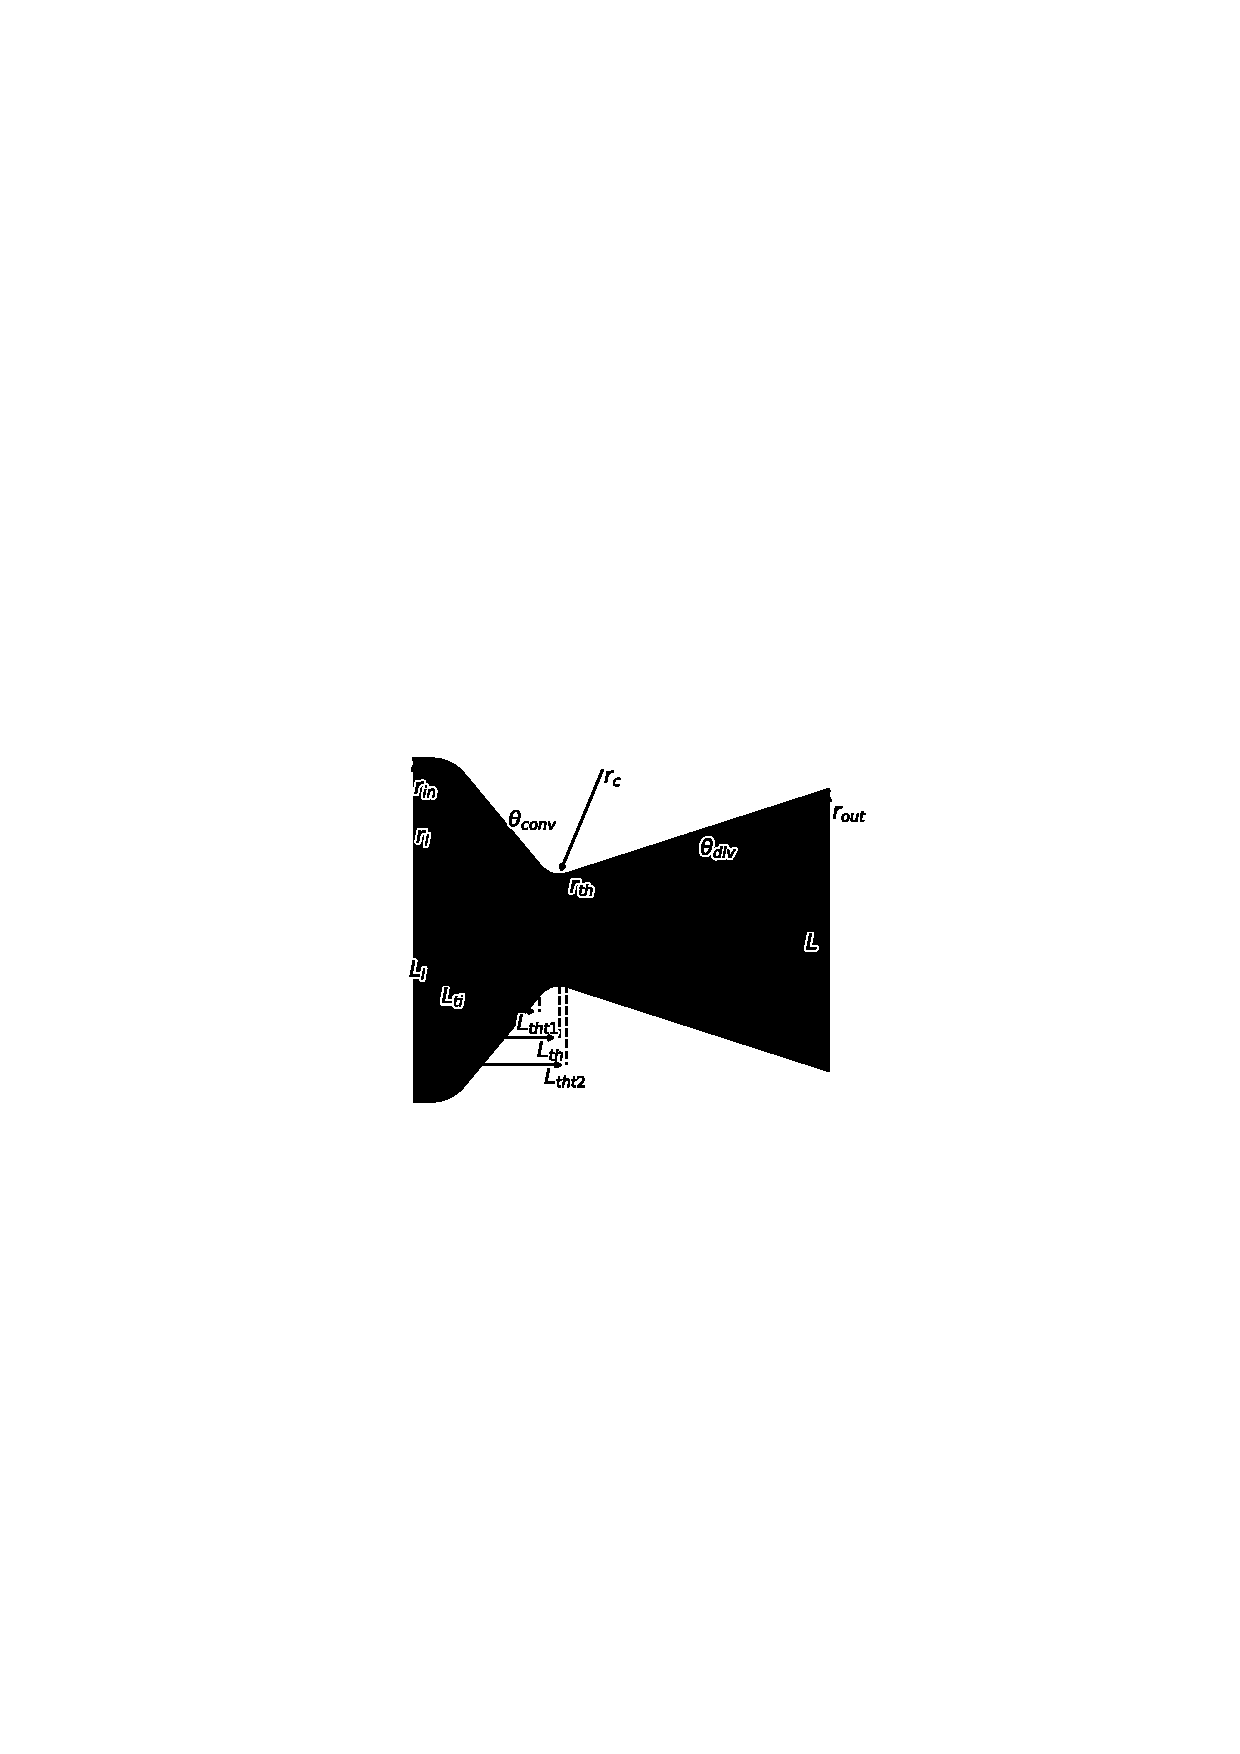
\includegraphics[width=0.50\linewidth]{Figuras/geometry_figures/nozzle_15_xy.pdf}
        \caption{Parametrized nozzle geometry.}
        \label{fig:geom_params}
\end{figure}

The geometry variability is obtained by varying the divergence angle $\theta_{div}$ and as a consequence the outlet radius $r_{out}$ while kepting the all remaining geometric paremeters constant. Such modification alter the area ratio after the troat as show in Figures \ref{fig:nozzle_10}, \ref{fig:nozzle_15} and \ref{fig:nozzle_20}, and is sufficient to impact the flow acceleration or deceleration, after the throat, determining if a shock is likely to form, and if it is the case the position of normal shock and structure of oblique shocks.

\begin{figure}[t]
    \centering
    \begin{subfigure}{0.3\textwidth}
        \centering
        % include second image
        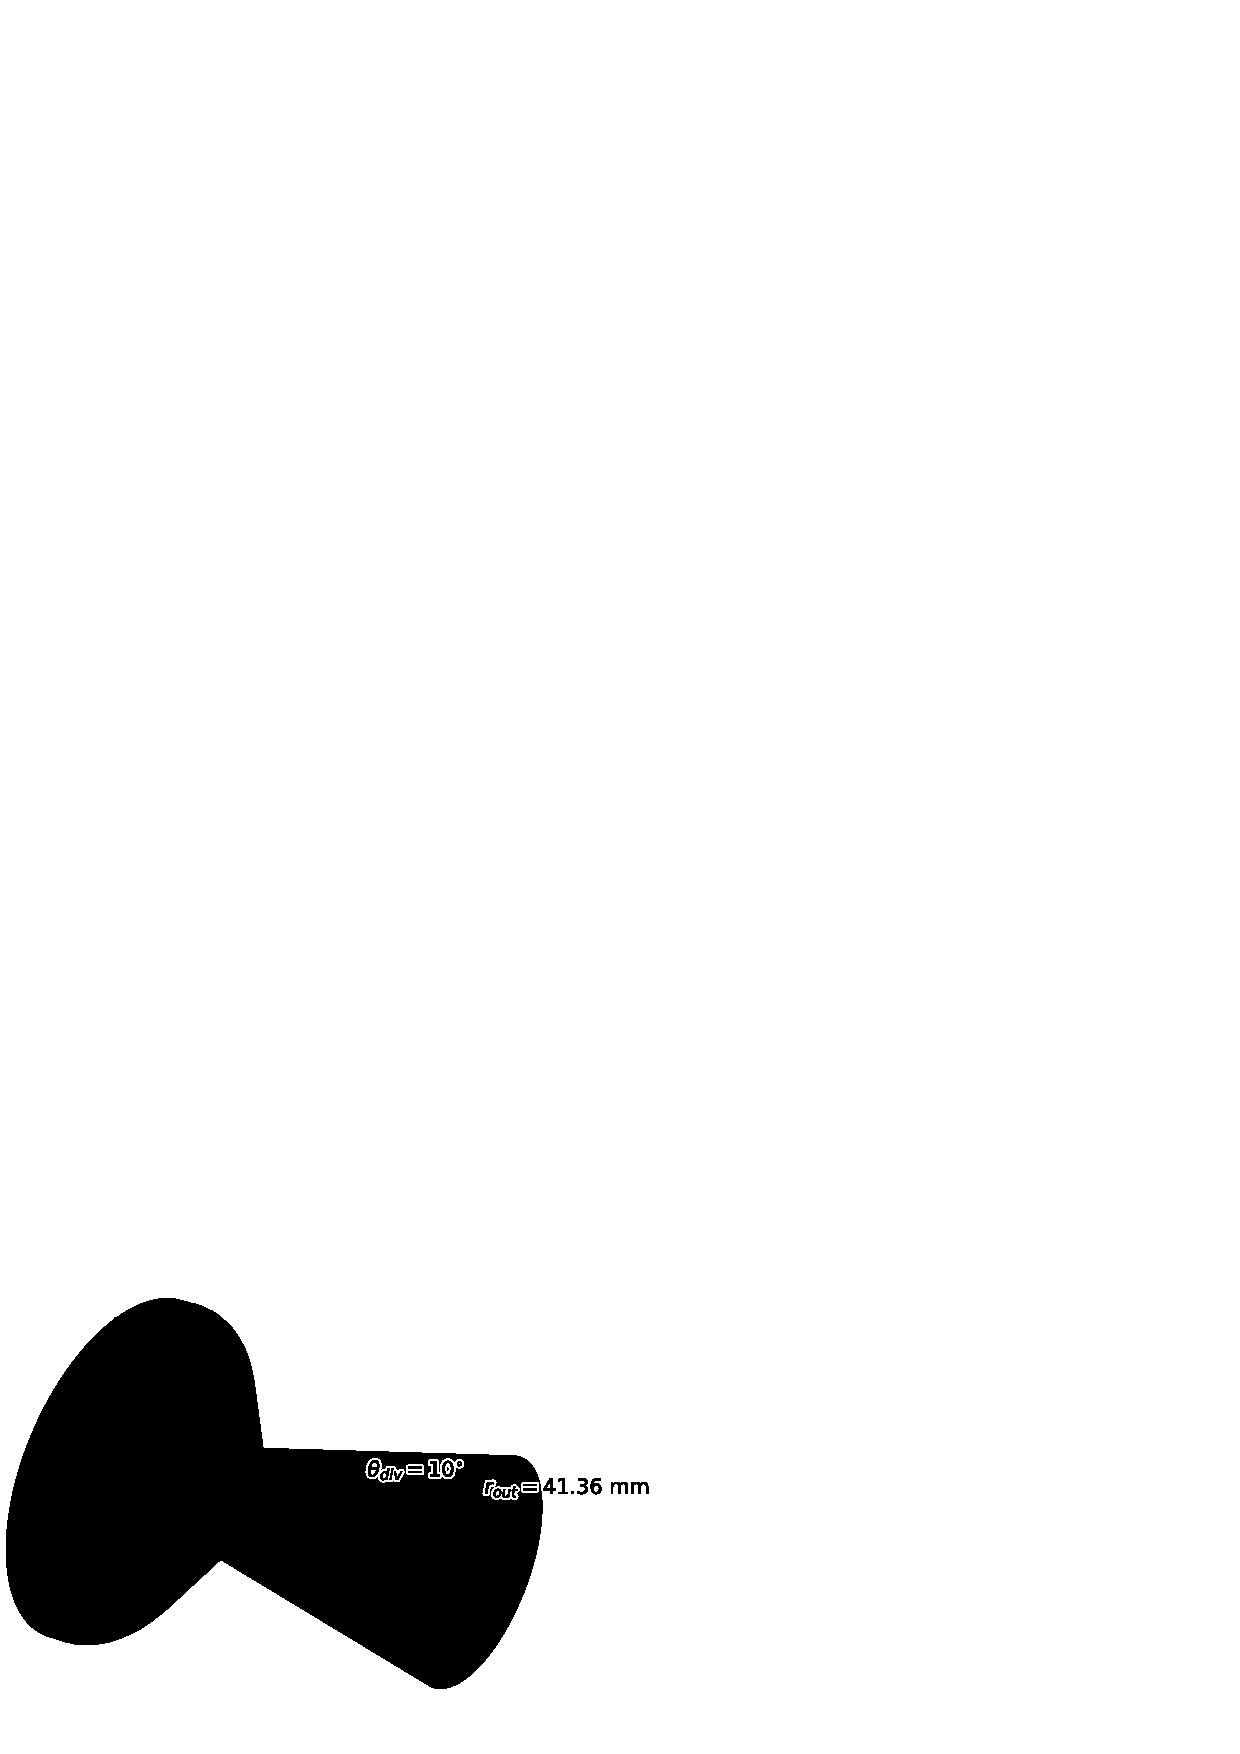
\includegraphics[width=\linewidth]{Figuras/geometry_figures/nozzle_10.pdf}  
        \caption{$\theta_{div}=10^{\circ}$.\label{fig:nozzle_10}}
    \end{subfigure}
    \begin{subfigure}{0.3\textwidth}
        \centering
        % include second image
        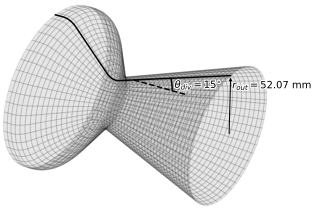
\includegraphics[width=\linewidth]{Figuras/geometry_figures/nozzle_15.pdf}  
        \caption{$\theta_{div}=15^{\circ}$.\label{fig:nozzle_15}}
    \end{subfigure}
    \begin{subfigure}{0.3\textwidth}
        \centering
        
\includegraphics[width=\linewidth]{Figuras/geometry_figures/nozzle_20.pdf}  
        \caption{$\theta_{div}=20^{\circ}$.\label{fig:nozzle_20}}
    \end{subfigure}
    \caption{Parametrized Nozzle geometries, (b) is the baseline.}
\end{figure}

The CAD model is encapsulated into an abstract class, from withinh the nozzle area variation is conputed to be input in thw low fidelity cfd model and also a numerical domain is build for the high fidelity model.

\section{Numerical Methods}

The \textit{low fidelity} solutions  were obtained using a finite volume solver for the steady-state Euler equations, with a detailed description provided in Section \ref{sec:q1d_euler}. This method saves computing time by assuming the flow to be non-viscous and the domain to be one-dimensional, with only the cross-sectional area of the nozzle allowed to vary along the symmetry axis.

For the \textit{high fidelity} solutions, the steady-state compressible Reynolds-Averaged Navier-Stokes equations were solved using the open-source finite volume solver SU2, with details of the implementation provided in Section \ref{sec:2d_navier_stokes_solver}. Due to intrinsic axisymmetry, the domain was assumed to be two-dimensional. This method is able to model turbulence effects using the shear stress transport closure, and also, boundary conditions other than adiabatic could be used on the nozzle walls.

\subsection{Quasi-1D Euler Solver}
\label{sec:q1d_euler}

The hot flowing air inside the nozzle is considered to be a compressible and calorically perfect gas. The set of equations for conservation of mass, momentum, and energy forms the well-known quasi-1D Euler equations, written compactly in vector notation as Equation \eqref{eq:q1d_euler_vec}.

\begin{equation}
    \symbl{$\partial$}{Partial derivative}
    \frac{\partial}{\partial t}{\mathbf{U}}  + \frac{\partial }{\partial x}\mathbf{F} = \mathbf{S} 
    \label{eq:q1d_euler_vec}
\end{equation}

Denoting the primitive variables specific mass as $\rho$, x-component velocity as $u$, pressure as $p$, and the specific total energy as $e$, and with the cross-sectional area denoted as $A$, these vectors are formed as shown in Equation \eqref{eq:q1d_euler_vectors}.

\begin{eqnarray}
    \symbl{$\partial$}{Partial derivative}
    \mathbf{U} = \begin{bmatrix} \rho \\ \rho u \\ e \end{bmatrix} & \mathbf{F} = \begin{bmatrix} \rho u \\ \rho u^2 + p \\ (e+p)u \end{bmatrix} & \mathbf{S} = \begin{bmatrix} 0 \\ \frac{p}{A} \frac{dA}{dx} \\ 0 \end{bmatrix}
    \label{eq:q1d_euler_vectors}
\end{eqnarray}

A steady state numerical solution for this system of equations is found by usign a time marching numerical scheme, as in equation \eqref{eq:time_marching}

\begin{equation}
   \mathbf{U}^{n+1} = \mathbf{U}^{n} + \Delta t^n \mathbf{R} (\Delta t^n, U^n) 
   \label{eq:time_marching}
\end{equation}

, the residual, \eqref{eq:q1d_euler_res}, for each time step is computed using a finite volume method discretization over the 1D domain, represented graphically in Figure \ref{fig:1d_domain}.

\begin{figure}
\centering
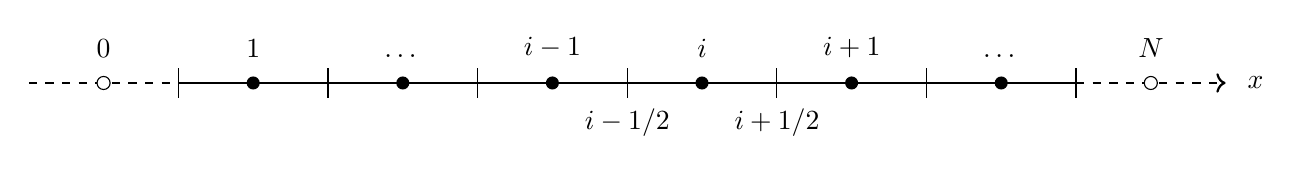
\begin{tikzpicture}[scale=1.9]
	\draw [thick] (0,0) -- (6,0);
	\draw [dashed,thick] (-1,0) -- (0,0);
	\draw [->,dashed,thick] (6,0) -- (7,0);

	\node at (7.2,0) {$x$};

    \def\celllabel[#1](#2){
        \node[fill=black,circle, scale=0.0, label={[yshift=2mm]above:$#2$}] at (#1+0.5,0) {};
    }

    \def\cell(#1){
        \node[fill=black,circle, scale=0.5] at (#1+0.5,0) {};
    }

    \def\ghostcell(#1){
        \node[circle, draw=black, fill=white, scale=0.5] at (#1+0.5,0) {};
    }

    \def\face(#1){
        \draw (#1,0.1) -- (#1, -.1); 
    }

    \def\facelabel[#1](#2){
        \node[scale=0.0, label={[yshift=-2mm]below:$#2$}] at (#1,0) {};
    }

    % draw faces
	\foreach \i in {0,1,...,6}{
		\face(\i);	
	}

    % draw face labels
    \facelabel[3](i-1/2);
    \facelabel[4](i+1/2);

    % draw cell centers
    \foreach \i in {0,1,...,5}{
        \cell(\i);
	}

    % draw ghost cells
    \ghostcell(-1);
    \ghostcell(6);

    % draw cell labels
    \celllabel[-1](0);
    \celllabel[0](1);
    \celllabel[1]($\ldots$);
    \celllabel[2](i-1);
    \celllabel[3](i);
    \celllabel[4](i+1);
    \celllabel[5]($\ldots$);
    \celllabel[6](N);
\end{tikzpicture}
\label{fig:1d_domain}
\caption{Quasi one dimensional domain discretization for the cell-centered finite volume method.}
\end{figure}

\begin{equation}
\mathbf{R}(\Delta t^n, U^n) = \mathbf{S}_i^n - \frac{1}{\Delta x_i} \left( \mathbf{F}^{n}_{i+1/2} - \mathbf{F}^{n}_{i-1/2} \right) 
\label{eq:q1d_euler_res}
\end{equation}

The system of equations is then integrated in time using a 4th-order Runge-Kutta scheme, whit timestep $\Delta t$ determined by imposiv a CFL number

\begin{align}
    k_1 &= \mathbf{R}(t^n, U^n)  \\
    k_2 &= \mathbf{R}(t^n + \frac{\Delta t^n}{2}, U^n +  \Delta t^n \frac{k_1}{2}) \\
    k_3 &= \mathbf{R}(t^n + \frac{\Delta t^n}{2}, U^n +  \Delta t^n \frac{k_2}{2}) \\
    k_4 &= \mathbf{R}(t^n + \Delta t^n, U^n + \Delta t^n k_3) \\
    \mathbf{U}^{n+1} &= \mathbf{U}^n + \frac{1}{6}(k_1 + 2k_2 + 2k_3 + k_4)
\end{align}

The quasi one-dimensional numerical method used in this work is an in-house cfd solver for the compressible Euler equations \eqref{eq:q1d_euler_vec}. Altough the method can capture compressible effects and shock formation, the shock is sharper than the viscous one. The method is also unable to predict the diamond structure of oblique shocks. The method also does not take into account any prescribed tempeture in the wall. 

\subsubsection{Numerical Verification and Validation}

To evaluate the validity of the method, results from our implementation was compered with numerical results obtained by

NUMERICAL VALIDATAION/VERIFICATION

\subsection{2D Navier-Stokes Solver}
\label{sec:2d_navier_stokes_solver}

The compressible Navier-Stokes equation \eqref{eq:ns_equations} was solved in 2D.

\begin{equation}
    \mathbf{R(\mathbf{U})} = \frac{\partial \mathbf{U}}{\partial t} + \nabla \cdot \mathbf{F}^c(\mathbf{U}) - \nabla \cdot \mathbf{F}^v(\mathbf{U}, \nabla \mathbf{U}) - \mathbf{S}
    \label{eq:navier-stokes}
\end{equation}


\begin{eqnarray}
   %\symbl{$\partial$}{Partial derivative}
   \mathbf{U} = \begin{bmatrix} \rho \\ \rho \mathbf{v} \\ \rho E \end{bmatrix} 
   & \mathbf{F}^c = \begin{bmatrix} \rho \mathbf{v}  \\ \rho \mathbf{v}\otimes \mathbf{v} + \mathbf{1} p \\ \rho E \mathbf{v} + p \mathbf{v} \end{bmatrix} 
   & \mathbf{F}^v = \begin{bmatrix} \cdot \\ \boldsymbol{\tau} \\ \boldsymbol{\tau} \cdot \mathbf{v} + \kappa \nabla T \end{bmatrix} 
   %& \mathbf{S} = \begin{bmatrix} 0 \\ 0  \\ 0 \end{bmatrix}
   \label{eq:ns_equations}
\end{eqnarray}

, with a viscous stress tensor given by 

\begin{equation}
    \boldsymbol{\tau} = \mu \left( \nabla \mathbf{v} + \nabla \mathbf{v}^T \right) - \mu \frac{2}{3} \mathbf{1} \left( \nabla \cdot \mathbf{v} \right)
    \label{eq:ns_stress_tensor}
\end{equation}

The viscosity is

\begin{equation}
    \mu = \mu_d + \mu_t
    \label{eq:mu}
\end{equation}

and the thermal conductivity

\begin{equation}
    \kappa = \frac{\mu_d + c_p}{Pr_d} + \frac{\mu_t c_p}{Pr_t}
    \label{eq:kappa}
\end{equation}

where $\rho$ is the fluid density, $\mathbf{v} = \left\{ u , v \right\}^T \in \mathbb{R}$ is the flow velocity vector, with $u$ and $v$ being its components. $E$ is the total energy per unit mass, $p$ the static pressure, $\boldsymbol{\tau}$ the viscous stress tensor, $T$ the static temprature, $\kappa$ the thermal conductivity, and $\mu$ the viscosity.

With an assumption of a perfect gas, with constant specific heat ratios $\gamma$, and gas constant $R$, the system can be closed using the relation for pressure

\begin{equation}
    p = \rho \left( \gamma - 1 \right) \left[ E - \frac{1}{2} \left( \mathbf{v} \cdot \mathbf{v} \right) \right]
    \label{eq:pressure}
\end{equation}

The SU2 software \cite{Economon2016a} was employed, the Reynolds Averaged Navier-Stokes equations were solved using the finite volume method and the SST (Shear Stress Transport) turbulence model. To obtain the steady-state solution, the implicit Euler integration method was utilized in conjunction with time marching.

\subsubsection{Grid Independence Study}

A Grid Independence Study using the Grid Convergence Index (GCI) \cite{Roache1994} was performed to assess numerical accuracy. Table 1 lists the three mesh levels used and Table 2 shows the results. Positive p and small GCI values indicate a monotonic and asymptotic convergence, respectively. A GCIasymptotic close to 1 indicates grid-independent solutions, so Medium was chosen for further analysis (shown in Figure 2).

\begin{table}
\centering
\begin{tabular}{lccccccc}
\toprule
        & $ \bar{p} $ & $ N_{cells} $ & $ r $ & $ GCI $ & $ \bar{p}_{extrapolated} $ & $ order $ &  $ GCI_{asymp.} $ \\ \midrule
Fine    & $9.995\times10^4$ & $6000$  & $1.5$ & $0.17$ \% &  \multirow{3}{*}{$1.00\times10^5$} &  \multirow{3}{*}{$1.99$} &  \multirow{3}{*}{$1.002$} \\ 
Medium  & $9.980\times10^4$ & $2500$  & $1.3$ & $0.41$ \% & & & \\ 
Coarse  & $9.950\times10^4$ & $1500$  & -     & -         & & & \\ 
        & $ \bar{T} $ & $ N_{cells} $ & $ r $ & $ GCI $ & $ \bar{T}_{extrapolated} $ & $ order $ &  $ GCI_{asymp.}$ \\ \midrule 
Fine    & $6.909\times10^2$ & $6000$  & $1.5$ & $0.00$ \% &  \multirow{3}{*}{$6.91\times10^2$}  &   \multirow{3}{*}{$8.14$} &   \multirow{3}{*}{$1.000$} \\ 
Medium  & $6.910\times10^2$ & $2500$  & $1.3$ & $0.04$ \% & & & \\ 
Coarse  & $6.930\times10^2$ & $1500$  & -     & -         & & & \\ 
\bottomrule
\end{tabular}
\caption{Grid convergence study over 3 grids.}
\label{tab:gci_study}
\end{table}

\begin{figure}[h]
  \centering
  \includegraphics[width=\linewidth]{Figuras/validation/validation_medium.pdf}
  \caption{Validation using all experimental data of reference \cite{Back1965a} for the nozzle in question.}
  \label{fig:validation_su2}
\end{figure}

\section{Design of Eperiments}

As the method is data driven, data must be gattered or generated. In this study three distincts datasets was generated using a Latin Hypercube Sampling using 1000 iterations to maximize the minimal \textit{pdist}. The ranges for the independent variables is described in Table \ref{tab:doe_lhs}. The surrogate model should be able to reconstruct any flow field of simulations within the precribed design of experiment space of parameters. The dataset consist onluy of converged simulations, the convergence criteria utilized is the maximum residue of $10^{-8}$ for the mass, momementum and energy equation. The dataset was also split into training, validation and test, using $90$ \% of total data for training, 5 \% for validation and the remaining 5 \% for testing.

\begin{table}[h!]
  \centering
  \begin{tabular}{lrlcccc} 
   \toprule
   \multirow[b]{3}{*}{\makecell[l]{Wall \\ Boundary \\ Condition}} & \multirow[b]{3}{*}{\makecell[r]{Dataset \\ Size}} &  \multirow[b]{3}{*}{\makecell[l]{\makecell[l]{(Training, \\Validation, \\Test)} }} & \multicolumn{4}{c}{Independent Parameters} \\
    &  & & $p_0$ [MPa] & $T_0$ [K] & $\theta_{div}$ [$^\circ$] & $T_w$ [K]\\
    &  &  & \makecell{(min,\\max)} & \makecell{(min,\\max)} & \makecell{(min,\\max)} & \makecell{(min,\\max)} \\
   \midrule
   \multirow{3}{*}{\makecell[l]{Prescribed \\ Temperature}} & Small & $(130,17,16)$ & \multirow{3}{*}{\makecell{$(0.35$,\\$1.70)$}} & \multirow{3}{*}{\makecell{$(300.00,$\\$ 800.00)$}} & \multirow{3}{*}{\makecell{$(10.00$,\\$20.00)$}} & \multirow{3}{*}{\makecell{$(120.00$,\\$300.00)$}} \\ 
   & Medium & $(332,42,41)$ &  &  & & \\
   & Large & $(652,82,82)$ &  &  & & \\
   \midrule
   \multirow{3}{*}{Adiabatic} & Small & $(128,17,16)$ & \multirow{3}{*}{\makecell{$(0.35$,\\$1.70)$}} & \multirow{3}{*}{\makecell{$(300.00,$\\$ 800.00)$}} & \multirow{3}{*}{\makecell{$(10.00$,\\$20.00)$}} &  \\ 
   & Medium & $(323,41,40)$ &  &  & & \\
   & Large & $(644,81,81)$ &  &  & & \\ 
   \bottomrule
  \end{tabular}
  \caption{Dataset ranges for design variables and final dataset sizes retaining converged simlation.}
  \label{tab:doe_lhs}
\end{table}

Since our method relies entirely on data, where the data comes from doesn't matter—it could be gathered through experiments or artificially created using any numerical method. In this study, we're using synthetic data because it makes it easy and quick to control numerical experiments, especially in terms of the number of experiments and the quality of the data.

Regardless of the situation, the first step is to gather two sets of data: one with low fidelity and the other with high fidelity. The low-fidelity data could be a simulation with a rough grid, shortened dimensions, or other simplifications, and it might only include global scalar variables like geometry parameters and averaged boundary conditions. In the world of fluid dynamics, the high-fidelity dataset usually involves multidimensional simulations, trying to capture as much of the physics as possible.

\begin{figure}[t]
    \centering
    \begin{subfigure}{0.3\textwidth}
        \centering
        % include second image
        \includegraphics[width=\linewidth]{Figuras/lhs/data_adiabatic/doe_200/lhs_all.pdf}  
        \caption{Small dataset.}
        \label{fig:lhs_adiabatic_200}
    \end{subfigure}
    \begin{subfigure}{0.3\textwidth}
        \centering
        % include second image
        \includegraphics[width=\linewidth]{Figuras/lhs/data_adiabatic/doe_500/lhs_all.pdf}  
        \caption{Medium dataset.}
        \label{fig:lhs_adiabatic_500}
    \end{subfigure}
    \begin{subfigure}{0.3\textwidth}
        \centering
        \includegraphics[width=\linewidth]{Figuras/lhs/data_adiabatic/doe_1000/lhs_all.pdf}  
        \caption{Large dataset.}
        \label{fig:lhs_adiabatic_1000}
    \end{subfigure}
    \caption{Latin Hypercube Sampling for Design of Experiments with adiabatic wall.}
    \label{fig:lhs_adiabatic}
\end{figure}

\begin{figure}[t]
    \centering
    \begin{subfigure}{0.3\textwidth}
        \centering
        % include second image
        \includegraphics[width=\linewidth]{Figuras/lhs/data_Tw/doe_200/lhs_all.pdf}  
        \caption{Small dataset.}
        \label{fig:lhs_Tw_200}
    \end{subfigure}
    \begin{subfigure}{0.3\textwidth}
        \centering
        % include second image
        \includegraphics[width=\linewidth]{Figuras/lhs/data_Tw/doe_500/lhs_all.pdf}  
        \caption{Medium dataset.}
        \label{fig:lhs_Tw_500}
    \end{subfigure}
    \begin{subfigure}{0.3\textwidth}
        \centering
        \includegraphics[width=\linewidth]{Figuras/lhs/data_Tw/doe_1000/lhs_all.pdf}  
        \caption{Large dataset}
        \label{fig:lhs_Tw_1000}
    \end{subfigure}
    \caption{Latin Hypercube Sampling for Design of Experiments with prescribed wall temperature.}
    \label{fig:lhs_Tw}
\end{figure}

\section{Dimensionality Reduction Study}


\subsection{Dimensionality Reduction}

The flow reconstruction technique is specifically devised for addressing fluid flow fields, where the number of degrees of freedom is intricately tied to the elements in a full-order numerical simulation. In 3D flow fields, this association can result in an exceedingly large number of degrees of freedom, often reaching millions or even billions. Even in the context of the simplified 2D numerical simulation presented in this study, the number of degrees of freedom is on the order of $10^4$. This numerical value signifies the variables that the surrogate model must encapsulate. Therefore, any reduction in this count not only reflects a judicious application of compressed data but also yields a more cost-effective model.

In addition to the computational efficiency gained by diminishing the computational burden required for modeling the flow field, the process of dimensionality reduction also enhances the model's fitting capabilities. This is owing to the substantial reduction in the number of coupled linear equations that need to be modeled. In essence, the streamlined approach not only contributes to computational economy but also augments the model's efficacy in representing the underlying fluid dynamics.

To enact data compression, the matrices that compile training snapshots for low-fidelity and high-fidelity simulations, denoted as $\mathbf{X}_{l}$ and $\mathbf{X}_h$ respectively, underwent compression utilizing the truncated Singular Value Decomposition (SVD) technique. In essence, the SVD factorization, expressed in equation \ref{eq:svd}, possesses the capability to precisely represent any matrix $\mathbf{X}$ if the number of elements in the diagonal of the square singular values matrix $\mathbf{\Sigma}$ equals the original rank of the matrix $\mathbf{X}$. 

\begin{equation}
    \mathbf{X} = \mathbf{U}\mathbf{\Sigma}\mathbf{V}^T  
    \label{eq:svd}
\end{equation}

Data compression is then achieved by truncating the number of singular values, retaining only the most significant ones, those with higher absolute values arranged in decreasing order. This process serves to distill essential information from the matrices, offering an effective means of compression while maintaining fidelity to the underlying data structure.

\subsection{Projection Error Analysis}

It is a commonplace procedure to determine the appropriate number of singular values for truncation by assessing the energy or explained variance of the reconstructed matrix $\mathbf{\tilde{X}}$ following reprojection with a truncated basis. However, our investigations reveal that this method is less effective than evaluating the sensitivity of surrogate model accuracy concerning the number of principal components employed. This is due to the fact that a more accurate basis does not necessarily correspond to a more accurate surrogate. To gauge model sensitivity regarding the number of principal components utilized, a series of numerical studies was undertaken. Kriging served as the surrogate model in these studies, with the objective of identifying the minimal number of principal components required to maintain high accuracy.

The search space for this study is the truncated rank of SVD decomposition for the low and high fidelity simulation datasets. The maximum allowed rank is determined by the full matrix of snapshots rank, and could be bounded by the number of samples or the full dimension of each sample. 

\subsection{Grid Search}

A dimensionality reduction study was conducted to investigate the performance of the reduced order models with respect to the input and output dimensions in terms os R2, NRMSE and MAPE metrics. The Gaussian Process was used to map from the input space to the output space. A simple grid search algorithm was used to find the optimal pair of input and output dimensions.

\begin{algorithm}
    \caption{Grid Search Algorithm in trial space $\Omega = \left\{\mathcal{N_X}, \mathcal{N_Y}\right\} $}
    \label{alg:grid_search}
    \begin{algorithmic}[1]
        \Require{trials for input dimension $\mathcal{N_X}=\{{n_{\mathcal{X}}}_1, \ldots, {n_{\mathcal{X}}}_N\}$; trials for output dimension $\mathcal{N_Y}=\{{n_{\mathcal{Y}}}_1, \ldots, {n_{\mathcal{Y}}}_M\}$; training functions $\mathcal{F}$,  metric evalators $\mathcal{M}=\{m_1, \ldots, m_K\}$}
        \Ensure{Tensor of metrics $\mathcal{M}$ and hyperparameters $\boldsymbol{\mu}$}
        \State $i \gets 1$
        \State $j \gets 1$
        \For {${n_{\mathcal{X}}}_i \in \mathcal{N_X}$}
            \For {${n_{\mathcal{Y}}}_j \in \mathcal{N_Y}$}
                \State $\boldsymbol{\mu} \gets \boldsymbol{\mu}_0 \cup \{{n_{\mathcal{X}}}_i,  {n_{\mathcal{Y}}}_j\}$
                \State $\mathbf{\Phi} \gets  \mathcal{F}(\mathbf{\Phi},\mathbf{X}_{tr}, \mathbf{y}_{tr} , \boldsymbol{\mu})$
                \State $\tilde{\mathbf{y}} \gets \mathbf{\Phi}(\mathbf{X}_{te})$
                \State $k \gets 1$
                \For {$m_k \in \mathcal{M}$}
                    \State $\mathbf{\Xi}(i,j) \gets \mathbf{\Xi}(i,j) \cup m_k(\mathbf{y}_{te}, \tilde{\mathbf{y}})$
                    \State $k \gets k + 1$
                \EndFor
                \State $\mathbf{\Xi}(i,j) \gets \mathbf{\Xi}(i,j) \cup \boldsymbol{\mu}$     
                \State $i \gets i + 1$
            \EndFor
            \State $j \gets j + 1$
        \EndFor
    \end{algorithmic}
\end{algorithm}

\plotdrs{data_Tw}{fields}{MAPE}{MAPE for prediction using only one dimensional fields.}

\plotdrs{data_Tw}{fields}{NRMSE}{NRMSE for prediction using only one dimensional fields.}

\plotdrs{data_Tw}{fields}{R2}{R2 for prediction using only one dimensional fields.}

\plotdrs{data_adiabatic}{fields}{MAPE}{MAPE for prediction using only one dimensional fields, adiabatic wall.}

\plotdrs{data_adiabatic}{fields}{NRMSE}{NRMSE for prediction using only one dimensional fields, adiabatic wall.}

\plotdrs{data_adiabatic}{fields}{R2}{R2 for prediction using only one dimensional fields, adiabatic wall.}

% \begin{table}[h!]
%     \centering
%     \begin{tabular}{c c c c c}
%     \toprule
%     \textbf{Input} & \textbf{Dataset Size} & \textbf{NRMSE} & \textbf{R2} & \textbf{MAPE} \\
%     \midrule
%     \addlinespace[1em]
%     \multirow[b]{3}{*}{$\begin{bmatrix}p \\ T \\ M \\ A \\ T_{wd}\end{bmatrix}$} & Small & 0.01 & 0.98 & 0.01 \rule{0pt}{5pt} \\
%     \addlinespace[1em]
%     & Medium & 0.01 & 0.98 & 0.01 \\
%     \addlinespace[1em]
%     & Large & 0.01 & 0.98 & 0.01 \\
%     \addlinespace[1em]
%     \midrule 
%     \addlinespace[1em]
%     \multirow[b]{3}{*}{$\begin{bmatrix}p_0 \\ T_0 \\ T_w \\ \theta_{div}\end{bmatrix}$} & Small & 0.01 & 0.98 & 0.01 \\
%     \addlinespace[1em]
%     & Medium & 0.01 & 0.98 & 0.01 \\
%     \addlinespace[1em]
%     & Large & 0.01 & 0.98 & 0.01 \\
%     \addlinespace[1em]
%     \bottomrule
%     \end{tabular}
% \end{table}

\begin{table}[h!]
    \centering
    \begin{tabular}{c c c c c} 
     \toprule
     \textbf{Input} & \textbf{Dataset Size}  &\textbf{Input Components} &  \textbf{Output}  & \textbf{Output Components}\\ 
     \hline
     \hline
     \multirow{15}{*}{$\begin{bmatrix} p \\ T \\ M \\ A \\ T_{wd} \\ p_0 \\ T_0 \\ T_w \\ \theta_{div} \end{bmatrix}^{}$ } & \multirow{5}{*}{Small}  & \multirow{5}{*}{\{2,7,12,...,162\}} & $\begin{bmatrix} p \end{bmatrix}$    & \multirow{4}{*}{\{2,7,12,...,162\}} \\ 
                            & &                                     & $\begin{bmatrix} T \end{bmatrix}$ & \\ 
                            & &                                     & $\begin{bmatrix} M \end{bmatrix}$        & \\ 
                            & &                                     & $\begin{bmatrix} p & T & M & q \end{bmatrix}$  & \\ \cline{4-5}
                            & &                                     & $\begin{bmatrix} q \end{bmatrix}$   & \{2,7,12,...,98\} \\ \cline{2-5}
                        
      & \multirow{5}{*}{Medium} & \multirow{5}{*}{\{2,7,12,...,418\}} & $\begin{bmatrix} p \end{bmatrix}$    & \multirow{4}{*}{\{2,7,12,...,418\}} \\ 
                            & &                                     & $\begin{bmatrix} T \end{bmatrix}$ & \\ 
                            & &                                     & $\begin{bmatrix} M \end{bmatrix}$       & \\ 
                            & &                                     & $\begin{bmatrix} p & T & M & q \end{bmatrix}$  & \\ \cline{4-5}
                            & &                                     & $\begin{bmatrix} q \end{bmatrix}$   & \{2,7,12,...,98\} \\ \cline{2-5}

     & \multirow{5}{*}{Large} & \multirow{5}{*}{\{2,7,12,...,497\}} & $\begin{bmatrix} p \end{bmatrix}$    & \multirow{4}{*}{\{2,7,12,...,794\}} \\ 
                            & &                                     & $\begin{bmatrix} T \end{bmatrix}$ & \\ 
                            & &                                     & $\begin{bmatrix} M \end{bmatrix}$        & \\ 
                            & &                                     & $\begin{bmatrix} p & T & M & q \end{bmatrix}$ & \\ \cline{4-5}
                            & &                                     & $\begin{bmatrix} q \end{bmatrix}$   & \{2,7,12,...,98\} \\
    \hline
    \end{tabular}
    \caption{Table to test captions and labels.}
    \label{table:1}
\end{table}


\section{Hyperparameter Optimization}

\begin{table}[htbp]
    \centering
    \caption{Hyperparameter Search Space}
    \label{tab:hyperparameter_search_space}
    \begin{tabularx}{\textwidth}{r X}
    \toprule
    \textbf{Hyperparameter} & \textbf{Search Space} \\ \midrule
    \midrule
    Input Dimension & $[2,3, \ldots, 95]$ \\
    Output Dimension & $[2,3, \ldots, 95]$ \\
    Number of Layers & $[1,2,3,4,5,6,7,8,9,10]$ \\
    Neurons in Hidden Layers & $[2, 3, \ldots, 475]$ \\
    Activation Function & \textsc{tanh}, \textsc{relu}, \textsc{gelu}, \textsc{exponential},  \textsc{rhard_sigmoid}, \textsc{selu}, \textsc{elu}, \textsc{sigmoid}, \textsc{softmax}, \textsc{softplus}, \textsc{softsign}, \textsc{swish} \\
    \bottomrule
    \end{tabularx}
\end{table}

\plothpoboxplot{all}{all}{Hyperparameter optimization.}
\plothpoboxplot{all}{200}{Hyperparameter optimization.}
\plothpoboxplot{all}{500}{Hyperparameter optimization.}
\plothpoboxplot{all}{1000}{Hyperparameter optimization.}
\plothpoboxplot{adiabatic}{all}{Hyperparameter optimization.}
\plothpoboxplot{adiabatic}{200}{Hyperparameter optimization.}
\plothpoboxplot{adiabatic}{500}{Hyperparameter optimization.}
\plothpoboxplot{adiabatic}{1000}{Hyperparameter optimization.}
\plothpoboxplot{Tw}{all}{Hyperparameter optimization.}
\plothpoboxplot{Tw}{200}{Hyperparameter optimization.}
\plothpoboxplot{Tw}{500}{Hyperparameter optimization.}
\plothpoboxplot{Tw}{1000}{Hyperparameter optimization.}

\plothpomap{all}{all}{Hyperparameter optimization.}
\plothpomap{all}{200}{Hyperparameter optimization.}
\plothpomap{all}{500}{Hyperparameter optimization.}
\plothpomap{all}{1000}{Hyperparameter optimization.}
\plothpomap{adiabatic}{all}{Hyperparameter optimization.}
\plothpomap{adiabatic}{200}{Hyperparameter optimization.}
\plothpomap{adiabatic}{500}{Hyperparameter optimization.}
\plothpomap{adiabatic}{1000}{Hyperparameter optimization.}
\plothpomap{Tw}{all}{Hyperparameter optimization.}
\plothpomap{Tw}{200}{Hyperparameter optimization.}
\plothpomap{Tw}{500}{Hyperparameter optimization.}
\plothpomap{Tw}{1000}{Hyperparameter optimization.}

\plothpohistogram{all}{all}{Histogram and Surface.}
\plothpohistogram{all}{200}{Histogram and Surface.}
\plothpohistogram{all}{500}{Histogram and Surface.}
\plothpohistogram{all}{1000}{HHistogram and Surface.}
\plothpohistogram{adiabatic}{all}{Histogram and Surface.}
\plothpohistogram{adiabatic}{200}{Histogram and Surface.}
\plothpohistogram{adiabatic}{500}{Histogram and Surface.}
\plothpohistogram{adiabatic}{1000}{Histogram and Surface.}
\plothpohistogram{Tw}{all}{Histogram and Surface.}
\plothpohistogram{Tw}{200}{Histogram and Surface.}
\plothpohistogram{Tw}{500}{Histogram and Surface.}
\plothpohistogram{Tw}{1000}{Histogram and Surface.}

\section{Results}


\begin{table}[h!]
\centering
\begin{tabular}{c c c c c c}
    \toprule
    \textbf{\makecell{Wall \\ Boundary \\ Condition}} & \textbf{Dataset Size} & \textbf{Input Variables} & \textbf{NRMSE} & \textbf{MAPE} & \textbf{R2} \\
    \midrule
    %\multirow{2}{*}{Prescribed Temperature} & \mulirow{2}{*}{Small} & & & & \\
    \multirow{9}{*}{\makecell{Prescribed\\Temperature}} & \multirow{3}{*}{Small} & Scalars & 0.144 & 0.138 & 0.772 \\
     & & Fields & 0.144 & 0.138 & 0.773 \\
     & & Mixed & 0.147 & 0.138 & 0.751 \\
     & \multirow{3}{*}{Medium} & Scalars & 0.106 & 0.105 & 0.912 \\
     & & Fields & 0.106 & 0.105 & 0.912 \\
     & & Mixed & 0.092 & 0.106 & 0.900 \\
     & \multirow{3}{*}{Large} & Scalars & 0.060 & 0.080 & 0.954 \\
     & & Fields & 0.060 & 0.080 & 0.954 \\
     & & Mixed & 0.061 & 0.089 & 0.944 \\
    \multirow{9}{*}{Adiabatic} & \multirow{3}{*}{Small} & Scalars & 0.024 & 0.037 & 0.961 \\
    & & Fields & 0.025 & 0.036 & 0.963 \\
    & & Mixed & 0.022 & 0.033 & 0.963 \\
    & \multirow{3}{*}{Medium} & Scalars & 0.027 & 0.033 & 0.969 \\
    & & Fields & 0.028 & 0.034 & 0.968 \\
    & & Mixed & 0.024 & 0.032 & 0.966 \\
    & \multirow{3}{*}{Large} & Scalars & 0.019 & 0.022 & 0.984 \\
    & & Fields & 0.018 & 0.022 & 0.983 \\
    & & Mixed & 0.017 & 0.021 & 0.986 \\
    \bottomrule
\end{tabular}
\end{table}


\subsubsection{Hyperband Bayesian Optimization}


















% &&&&&\\
% &&&&&\\
% &\mulirow{3}{*}{Small}&&&&\\
% &&&&&\\
% &&&&&\\
% &\mulirow{3}{*}{Small}&&&&\\
% &&&&&\\
% &&&&&\\
% \multirow{9}{*}{Adiabatic} &\mulirow{3}{*}{Small}&&&\\   
% &&&&&\\
% &&&&&\\
% &\mulirow{3}{*}{Small}&&&&\\
% &&&&&\\
% &&&&&\\
% &\mulirow{3}{*}{Small}&&&&\\
% &&&&&\\
% &&&&&\\      

% ===================================================================
% ABSTRACT
% ===================================================================
\chapter*{Abstract}
\addcontentsline{toc}{chapter}{Abstract}

This study presents a machine learning-based surrogate modeling framework for reconstructing steady-state two-dimensional nozzle flows under varying flow and geometric conditions. The approach enables accurate prediction of high-fidelity viscous fields using low-dimensional inputs, such as scalar boundary conditions or quasi-one-dimensional (Q1D) solutions. To mitigate the challenges of training on high-dimensional data, Proper Orthogonal Decomposition (POD) is employed for dimensionality reduction, retaining dominant flow features while significantly lowering computational cost. Two regression strategies were investigated: Artificial Neural Networks (ANNs) and Gaussian Processes (GPs). A custom loss function was introduced for ANN models, combining mean squared error in both latent and reconstructed physical spaces, promoting accurate full-field recovery. Hyperparameter tuning was performed using Bayesian Optimization with Hyperband (BOHB), revealing that shallow ANNs with activation functions such as \textit{sigmoid}, \textit{hard sigmoid}, and \textit{swish} consistently yield optimal performance. Comprehensive evaluation across multiple datasets and boundary conditions demonstrated that ANNs generally achieve higher coefficients of determination ($R^2$), while GPs attain lower normalized root mean square error (NRMSE) under large, clean datasets. Robustness tests revealed that ANN models degrade more gracefully under input noise, whereas GPs are more sensitive but outperform ANNs when sufficient clean data are available. K-fold cross-validation confirmed the stability of ANNs in data-scarce regimes, and SHapley Additive exPlanations (SHAP) analysis provided physical insight by identifying the dominant influence of total pressure and the limited effect of wall temperature. This work provides valuable insights and practical guidelines for developing accurate and computationally efficient surrogate models in fluid dynamics.


% ===================================================================
% ACKNOWLEDGEMENTS
% ===================================================================
\chapter*{Acknowledgements}
\addcontentsline{toc}{chapter}{Acknowledgements}

We gratefully acknowledge the support of the RCGI—Research Centre for Greenhouse Gas Innovation, hosted by the University of São Paulo (USP) and sponsored by FAPESP—São Paulo Research Foundation (2014/50279-4 and 2020/15230-5) and Shell Brasil, and the strategic importance of the support given by ANP (Brazil's National Oil, Natural Gas, and Biofuels Agency) through the R\&D levy regulation. Also, the support of the UFABC—Federal University of ABC, which provides all the computational and physical infrastructure.


% ===================================================================
% TABLE OF CONTENTS, LISTS OF FIGURES AND TABLES
% ===================================================================
\tableofcontents
\listoffigures
\listoftables

% ===================================================================
% CHAPTER 1: INTRODUCTION
% ===================================================================
\chapter{Introduction}

\section{Motivation and Context}

This dissertation addresses the challenge of developing computationally efficient surrogate models to replace resource-intensive Computational Fluid Dynamics (CFD) solvers, particularly during the design and optimization phases of engineering projects. The final objective is to create tools for Project 77 of the Research Centre for Greenhouse Gas Innovation (RCGI), which focuses on designing a centrifugal compressor for carbon capture and storage applications. The high computational demands of CFD simulations in such projects pose a significant bottleneck, especially when extensive evaluations are required for design space exploration and optimization.

To address this challenge, this work explores machine learning-based models as a computatinal affordable alternative to CFD solvers. These models aim to provide fast and accurate predictions of flow fields while remains being sensitive to geometric variations and boundary conditions. 

To validate the proposed framework, preliminary studies were conducted on simpler CFD problems, such as compressible flow in convergent-divergent nozzles and the reconstruction of pressure and temperature fields over blades in NASA Rotor 37. These initial investigations provided valuable insights and served as a foundation for developing surrogate models tailored to the intricate demands of centrifugal compressor design.

\section{Expected Content in the Introduction of a Doctoral Thesis}

The introduction of a doctoral thesis typically serves as the foundation for the entire research work. It is expected to include the following elements:

\begin{itemize}
    \item \textbf{Background and Context:} Provide a brief overview of the research area, highlighting its importance and relevance in the broader scientific or engineering domain.
    \item \textbf{Motivation:} Clearly articulate the reasons for undertaking the research, emphasizing the gaps or challenges in the existing body of knowledge.
    \item \textbf{Problem Statement:} Define the specific problem or question that the thesis aims to address, ensuring it is well-scoped and researchable.
    \item \textbf{Objectives:} Outline the main goals of the research, specifying what the study seeks to achieve.
    \item \textbf{Contributions:} Summarize the novel aspects of the work and its expected impact on the field.
    \item \textbf{Thesis Structure:} Provide a roadmap of the thesis, briefly describing the content of each chapter to guide the reader.
\end{itemize}

These elements collectively set the stage for the research, ensuring the reader understands the significance, scope, and direction of the work.

\section{Problem Statement and Objectives}

This work proposes a data-driven framework for constructing and optimizing machine-learning-based reduced-order models (ML-ROMs) for flow field reconstruction. The objective is to build a parametric surrogate model capable of reconstructing the flow fields of a supersonic hot air stream within a convergent-divergent nozzle. The model must be able to accurately predict high-fidelity viscous fields from low-dimensional inputs, such as scalar boundary conditions or quasi-one-dimensional (Q1D) solutions.

The main objectives are:
\begin{itemize}
    \item To develop an ML-ROM framework to reconstruct 2D nozzle flow fields from low-dimensional inputs.
    \item To investigate and compare two regression strategies: Artificial Neural Networks (ANNs) and Gaussian Processes (GPs).
    \item To introduce and evaluate a novel loss function for ANNs that combines errors in the latent and physical spaces to improve reconstruction fidelity.
    \item To perform a systematic hyperparameter optimization to find the most effective model architectures.
    \item To rigorously evaluate the performance, robustness, interpretability, and computational efficiency of the developed models.
\end{itemize}

\section{Thesis Contributions}
The main contributions of this work are:
\begin{itemize}
    \item A surrogate modeling framework that reconstructs 2D viscous nozzle flows from low-dimensional inputs using POD-based dimensionality reduction.
    \item A comprehensive evaluation of Artificial Neural Networks (ANNs) and Gaussian Processes (GPs) with extensive hyperparameter tuning via BOHB.
    \item A novel loss function that improves ANN performance by combining latent and physical-space reconstruction errors.
    \item An in-depth analysis of model robustness to data variability (k-fold cross-validation) and input noise, showing the superiority of ANNs in non-ideal data scenarios.
    \item The use of SHAP analysis to reveal the importance of input features, aligning with physical principles and supporting the interpretability of predictions.
    \item The demonstration that surrogate models enable real-time inference, achieving speed-ups of up to $7374\times$ compared to CFD solvers.
\end{itemize}

\section{Thesis Outline}
The remainder of this thesis is organized as follows:
\begin{itemize}
    \item \textbf{Chapter 2} presents the theoretical background, covering the governing equations of fluid dynamics, the nozzle flow modeling, and the theoretical basis for the machine learning methods used.
    \item \textbf{Chapter 3} details the methodology, including the setup of the numerical experiments, the generation of the datasets, and the complete ML-ROM architecture, from preprocessing to hyperparameter optimization.
    \item \textbf{Chapter 4} presents and discusses the results, focusing on model evaluation, robustness, interpretability, computational efficiency, and analysis of the flow field reconstructions.
    \item \textbf{Chapter 5} concludes the work, summarizing the key findings, discussing the limitations, and suggesting directions for future research.
\end{itemize}

\chapter{Literature Review}
\label{chap:lit_review}

\section{Introduction}

This chapter provides a review of the relevant literature, establishing the context for the present work. It begins by outlining the computational challenges in modern fluid dynamics that motivate the development of surrogate models. It then surveys the application of Machine Learning (ML) to the field, with a specific focus on Reduced-Order Models (ROMs) for flow field reconstruction. The state-of-the-art concerning data-driven techniques, particularly those employing Artificial Neural Networks (ANNs) and Gaussian Processes (GPs), is discussed. Finally, this review identifies the specific gaps in the current body of knowledge that this thesis aims to address, thereby positioning its contributions within the broader scientific landscape.

\section{The Challenge of High-Fidelity Flow Simulation}

In modern aerothermodynamic design and optimization, a detailed understanding of the flow field is indispensable. Traditionally, this knowledge is acquired through high-fidelity numerical simulations, such as solving the Reynolds-Averaged Navier–Stokes (RANS) or Large Eddy Simulation (LES) equations. However, these simulations are often computationally expensive, sometimes prohibitively so, especially when numerous evaluations are required for design space exploration, uncertainty quantification, or optimization tasks. This computational bottleneck has spurred the development of surrogate models, which aim to preserve the high accuracy of detailed simulations while drastically reducing the computational cost.

\section{Machine Learning as a Solution in Fluid Dynamics}

Machine Learning (ML), a subfield of Artificial Intelligence, has emerged as a powerful paradigm for modeling complex physical phenomena where governing equations are either unknown or computationally difficult to solve, as is the case with turbulent compressible flows. As noted by researchers such as \citet{mendezChallenges2024}, \citet{Brunton2020}, and \citet{vinuesaEmerging2022}, ML has been successfully applied to a wide array of engineering problems. These applications include, but are not limited to:
\begin{itemize}
    \item Pattern recognition \citep{bishopPattern2006, Groun2022, Salehi2018}
    \item Classification tasks \citep{Wang2016}
    \item Optimization and design \citep{Bock2019, ferreiraEnsemble2018, Kianifar2020, Peters2023}
    \item Flow control \citep{Montans2019, talaeiBoundary2018}
    \item Uncertainty quantification \citep{chuDeep2024, pengApplying2024, liangLiquid2024}
\end{itemize}
Despite these successes, persistent challenges in the application of ML to physical systems remain, particularly concerning model selection, optimization, interpretability, and the generalization of models to unseen conditions.

\section{Reduced-Order Modeling (ROMs)}

Reduced-Order Models (ROMs) are a specific class of surrogate models designed to approximate the behavior of high-dimensional systems using a much smaller number of degrees of freedom. The fundamental goal of a ROM is to capture the most influential dynamics of the system, thereby enabling rapid and efficient predictions.

\subsection{Projection-Based ROMs and Proper Orthogonal Decomposition (POD)}

A cornerstone of many ROM strategies is Proper Orthogonal Decomposition (POD), a technique for data compression and feature extraction that is mathematically equivalent to Principal Component Analysis (PCA). As detailed by \citet{berkoozProper1993} and \citet{taira2017modal}, POD is used in fluid dynamics to identify a set of orthogonal basis functions, or "modes," that capture the maximum possible kinetic energy for any given number of modes. These modes represent the dominant, large-scale coherent structures within the flow.

By projecting the high-dimensional governing equations (e.g., Navier-Stokes) onto a low-dimensional subspace spanned by a truncated set of these POD modes, one can create a computationally inexpensive projection-based ROM. However, these models can struggle with accurately capturing highly nonlinear phenomena or advection-dominated flows.

\section{Data-Driven ROMs for Flow Field Reconstruction}

An alternative and increasingly popular approach is the use of purely data-driven, or non-intrusive, ROMs. These methods learn the mapping between system parameters and the solution field directly from a database of high-fidelity simulation results. Recent studies have demonstrated the immense potential of ML to reconstruct high-dimensional flow fields from reduced or simplified input representations, especially given the availability of large CFD datasets \citep{Zhang2023, Erichson2020b, Deng2021, cahalyPLICNet2024, champenoisMachine2024, xuSelfsupervised2023}. This thesis follows this data-driven paradigm, creating a machine-learning-based reduced-order model (ML-ROM) for flow field reconstruction.

\subsection{Surrogate Models: Artificial Neural Networks and Gaussian Processes}

Within the data-driven framework, various regression algorithms can be employed as the core surrogate model. This work focuses on two of the most prominent techniques: Artificial Neural Networks (ANNs) and Gaussian Processes (GPs).

\begin{itemize}
    \item \textbf{Artificial Neural Networks (ANNs)} are powerful function approximators inspired by the structure of the human brain. Their ability to model highly nonlinear relationships makes them well-suited for complex regression problems. They have been widely used in fluid dynamics for their universal approximation capabilities \citep{Berner2022, Czum2020, Kumar2020}.

    \item \textbf{Gaussian Processes (GPs)} are a nonparametric Bayesian method for regression. Instead of learning a single function, a GP learns a distribution over functions that are consistent with the training data. As described by \citet{rasmussenGaussian2006}, this provides a principled way to quantify prediction uncertainty, which is a significant advantage in many engineering applications \citep{Liu2020, Hasdiana2018a}.
\end{itemize}

\section{Research Gap and Thesis Contribution}

While the application of ML-ROMs for flow reconstruction is an active area of research, several gaps remain. Many existing studies focus on flows with simpler physics or do not perform a systematic optimization of the underlying ML model architecture and hyperparameters. Furthermore, rigorous analysis of model robustness to noisy data and a deep dive into the interpretability of the learned representations are often lacking.

This thesis aims to fill these gaps by extending prior work, such as that by \citet{Yu2019}, to a more challenging physical problem. The focus is on a geometry-sensitive nozzle flow characterized by significant heat transfer and nonlinear shock formation, including complex shock wave–boundary layer interactions (SWBLI) as investigated by \citet{martelliFlow2020}. The specific contributions of this work, which address the identified gaps, are:

\begin{enumerate}
    \item \textbf{A Novel Loss Function:} To enhance model fidelity, a new loss function for ANNs is introduced, which combines reconstruction errors in both the latent (POD coefficient) space and the physical space.

    \item \textbf{Systematic Hyperparameter Optimization:} The BOHB algorithm \citep{falknerBOHB2018} is employed to systematically and efficiently tune the surrogate models, moving beyond ad-hoc architecture selection.

    \item \textbf{Comprehensive Robustness and Stability Analysis:} Model variance is assessed through k-fold cross-validation, and robustness is evaluated by injecting noise into the input data and analyzing the model's response.

    \item \textbf{Physics-Based Interpretability:} SHAP analysis \citep{lundberg2017unified} is incorporated to understand the influence of input features on model predictions, providing physical insights into the learned representations and building trust in the surrogate model's predictions.
\end{enumerate}

By addressing these points, this research provides a comprehensive framework and practical guidelines for developing accurate, efficient, and reliable surrogate models for complex fluid dynamics problems.
% ===================================================================
% CHAPTER 2: THEORETICAL BACKGROUND
% ===================================================================
\chapter{Theoretical Background}

\section{Nozzle Flow Modeling}
The nozzle geometry was parametrically constructed based on the reference geometry of the "$45^\circ$–$15^\circ$" conical nozzle from \citet{Back1965a}. The geometric parameters are listed in Table \ref{tab:geom_params_tese_en}. Geometric variability is introduced by adjusting the divergence angle $\theta_{div}$.

\begin{table}[h!]
  \centering
  \caption{Geometric parameters for the baseline nozzle geometry.}
  \label{tab:geom_params_tese_en}
  \begin{tabular}{ l J{3.3}{3} l l }
    \toprule
    \textbf{Parameter} & \textbf{Value} & \textbf{Units} & \textbf{Description} \\
    \midrule
    $L_i$             & 7.874   & mm  & Distance to $r_i$ center  \\
    $L_{\text{tht1}}$ & 55.880  & mm  & Convergent $r_c$ tangency distance  \\
    $L_{\text{tht2}}$ & 68.148  & mm  & Divergent $r_c$ tangency distance  \\
    $L_{\text{th}}$   & 64.872  & mm  & Length to throat  \\
    $L_{ti}$          & 22.250  & mm  & Length to $r_i$ tangency  \\
    $L$               & 185.039 & mm  & Full nozzle length  \\
    $r_c$             & 12.700  & mm  & Convergent section curvature radius  \\
    $r_i$             & 20.320  & mm  & Inlet curvature radius  \\
    $r_{in}$          & 63.500  & mm  & Inlet radius  \\
    $r_{th}$          & 20.320  & mm  & Throat radius  \\
    $r_{out}$         & 63.298  & mm  & Outlet radius  \\
    $\theta_{div}$    & 15.000  & deg & Divergence angle  \\
    $\theta_{conv}$   & 45.000  & deg & Convergence angle  \\
    \bottomrule
  \end{tabular}
\end{table}

\section{Governing Equations}

\subsection{Quasi-1D Euler Equations (Low-Fidelity)}
The low-fidelity model is based on the quasi-one-dimensional (quasi-1D) Euler equations, which assume steady, inviscid, and axially symmetric compressible flow behavior. The vector form of the equations is:
\begin{equation}
    \frac{\partial \mathbf{U}}{\partial t} + \frac{\partial \mathbf{F}}{\partial x} = \mathbf{S}
\end{equation}
where $\mathbf{U}$, $\mathbf{F}$, and $\mathbf{S}$ are the vectors of conserved variables, flux, and the geometric source term, respectively. A finite volume method was used for the numerical solution.

\subsection{Navier-Stokes Equations (High-Fidelity)}
The high-fidelity model solves the two-dimensional Reynolds-Averaged Navier-Stokes (RANS) equations, which account for viscous and thermal effects. The conservative form reads:
\begin{equation}
  \mathbf{R}(\mathbf{U}) = \frac{\partial \mathbf{U}}{\partial t} 
  + \nabla \cdot \mathbf{F}^c(\mathbf{U}) 
  - \nabla \cdot \mathbf{F}^v(\mathbf{U}, \nabla \mathbf{U}) 
  - \mathbf{S}
\end{equation}
where $\mathbf{F}^c$ and $\mathbf{F}^v$ are the convective and viscous fluxes. The equations were solved using the open-source SU2 CFD solver, with the SST turbulence model. Verification and validation were performed through a Grid Convergence Index (GCI) analysis and comparison with experimental data.

\section{Model Order Reduction}

\subsection{Proper Orthogonal Decomposition (POD)}
POD is used to manage the high dimensionality of the flow field snapshots. It extracts a low-dimensional latent representation that preserves the most energetic modes of the data. The projection is obtained via the Singular Value Decomposition (SVD) of the snapshot matrix $\mathbf{X} = \mathbf{U} \boldsymbol{\Sigma} \mathbf{V}^T$, where the columns of $\mathbf{V}$ are the POD modes. The reduced representation is $\mathbf{\overline{X}} = \mathbf{X} \mathbf{V}_{n \times k}$, where $k \ll n$.

\section{Machine Learning Surrogate Models}

\subsection{Artificial Neural Networks (ANNs)}
ANNs are universal function approximators. We use a fully connected feedforward multilayer perceptron (MLP), whose architecture is a composition of layers that apply an affine transformation followed by a nonlinear activation function.

\subsection{Gaussian Processes (GPs)}
GP regression is a nonparametric Bayesian method that models distributions over functions. It assumes that the output values are jointly distributed as a multivariate Gaussian, defined by a mean function $\mathcal{M}$ and a covariance function (kernel) $\mathcal{K}$. We use an anisotropic Radial Basis Function (RBF) kernel.


% ===================================================================
% CHAPTER 3: METHODOLOGY
% ===================================================================
\chapter{Methodology}

\section{Framework Overview}
The proposed methodology is divided into an offline phase (model training) and an online phase (inference). Figure \ref{fig:grafico_abstrato_tese_en} summarizes the entire workflow.

\begin{figure}[h!]
    \centering
    % \includegraphics[width=\textwidth]{path/to/your/graphical_abstract_image.png}
    \caption{Graphical abstract of the proposed framework, showing the offline (training) and online (inference) stages. (Placeholder for Figure 11 from the manuscript)}
    \label{fig:grafico_abstrato_tese_en}
\end{figure}

\section{Data Generation and Numerical Experiments}
Synthetic datasets were generated using CFD simulations under two boundary condition scenarios: adiabatic wall and prescribed wall temperature. Latin Hypercube Sampling (LHS) was used to sample the input parameter space. Six distinct datasets were created, varying in size (small, medium, large) and input format (scalar or vector field). Each high-fidelity output snapshot has a dimension of $n_h = 7878$.

\section{ML-ROM Framework}

\subsection{Preprocessing and Scaling}
Input and output data are standardized using a slice-wise mean centering (for different physical quantities) and a `MaxAbsScaler` to scale the data to the $[-1, 1]$ interval.

\subsection{Dimensionality Reduction}
POD is applied to the preprocessed data. The number of retained modes, $k$, is chosen to preserve 99.99\% of the cumulative explained variance of the training data.

\subsection{Surrogate Regressors}
A regression function $\boldsymbol{\Phi}: \mathbb{R}^{k_l} \rightarrow \mathbb{R}^{k_h}$ is trained to map the projected inputs to the projected outputs.

\subsection{ANN Loss Function and Training}
An innovative hybrid loss function was formulated for ANN training, combining the error in the latent space and the error in the reconstructed physical space:
\begin{equation}
  \mathcal{L} = w_{\mathrm{recon}}\,\mathcal{L}_{\mathrm{reduced}} + (1 - w_{\mathrm{recon}})\,\mathcal{L}_{\mathrm{reconstructed}}.
\end{equation}
Training is performed using the AdamW optimizer with weight decay and a warmup-cosine decay learning rate schedule.

\subsection{Hyperparameter Optimization (HPO)}
Bayesian Optimization with Hyperband (BOHB) was used to find the optimal hyperparameter configuration for the ANNs. Table \ref{tab:hpo_search_tese_en} details the search space.

\begin{table}[h!]
  \caption{Hyperparameter search space used in BOHB tuning.}
  \label{tab:hpo_search_tese_en}
  \centering
  \begin{tabularx}{\linewidth}{r X}
  \toprule
  \textbf{Hyperparameter} & \textbf{Search Space} \\
  \midrule
  Number of Layers ($H$) & $[1, 2, \dots, 10]$ \\
  Neurons per Layer ($J_i$) & $[2, 3, \dots, 475]$ \\
  Activation Function & \textit{tanh}, \textit{relu}, \textit{GELU}, \textit{hard sigmoid}, \textit{selu}, \textit{elu}, \textit{sigmoid}, \textit{softmax}, \textit{softplus}, \textit{softsign}, \textit{swish} \\
  Weight Decay ($\lambda_{\text{wd}}$) & $[10^{-6}, 10^{-2}]$ \\
  Dropout Rate & $[0.01, 0.30]$ \\
  Learning Rate ($\eta_0$) & $[10^{-3}, 10^{-2}]$ \\
  \bottomrule
  \end{tabularx}
\end{table}


% ===================================================================
% CHAPTER 4: RESULTS AND DISCUSSION
% ===================================================================
\chapter{Results and Discussion}

\section{Hyperparameter Optimization}
The HPO analysis revealed that shallow networks (1–2 hidden layers) with a moderate number of neurons and activation functions like \textit{sigmoid}, \textit{softmax}, or \textit{hard sigmoid} consistently achieved the best performance, defined as $\text{NRMSE} < 0.10$ and $R^2 > 0.90$.

\section{Cross-Validation and Overfitting Assessment}
K-fold cross-validation ($k=5$) was used to assess generalization. The results (Table \ref{tab:kfold_results_tese_en}) showed that ANN models generally achieved higher and more stable $R^2$ values, while GP models yielded lower NRMSE on large, clean datasets but showed high variability in data-scarce regimes. This indicates that ANNs are more robust, while GPs are more accurate under ideal data conditions.

\begin{table}[h!]
\centering
\caption{Error metrics for 5-fold run, NRMSE and R$^2$, comparing both GP and ANN models.}
\label{tab:kfold_results_tese_en}
\begin{tabularx}{\linewidth}{r Y Y Y Y Y Y}
    \toprule
    \textbf{Dataset} & \multicolumn{2}{c}{\textbf{NRMSE}} & \multicolumn{2}{c}{\textbf{R$^2$}} \\
    & \textbf{GP} & \textbf{ANN}  & \textbf{GP} & \textbf{ANN} \\
    \midrule
    ADLF & 0.022 ± 0.002 & 0.026 ± 0.007 & 0.967 ± 0.007 & 0.972 ± 0.011  \\
    ADMF & 0.027 ± 0.003 & 0.035 ± 0.004 & 0.962 ± 0.004 & 0.969 ± 0.004  \\
    ADSF & 0.065 ± 0.027 & 0.074 ± 0.015 & 0.931 ± 0.018 & 0.938 ± 0.006  \\
    ADLS & 0.022 ± 0.001 & 0.029 ± 0.002 & 0.965 ± 0.007 & 0.962 ± 0.012  \\
    ADMS & 0.025 ± 0.004 & 0.037 ± 0.008 & 0.96 ± 0.004 & 0.961 ± 0.004  \\
    ADSS & 0.038 ± 0.009 & 0.039 ± 0.007 & 0.943 ± 0.012 & 0.934 ± 0.024 \\
    \midrule
    PTLF & 0.027 ± 0.002 & 0.03 ± 0.003 & 0.954 ± 0.027 & 0.969 ± 0.01 \\
    PTMF & 0.051 ± 0.039 & 0.042 ± 0.008 & 0.939 ± 0.015 & 0.955 ± 0.015  \\
    PTSF & 0.356 ± 0.192 & 0.074 ± 0.021 & 0.704 ± 0.074 & 0.876 ± 0.027  \\
    PTLS & 0.023 ± 0.001 & 0.03 ± 0.003 & 0.963 ± 0.01 & 0.967 ± 0.01  \\
    PTMS & 0.025 ± 0.005 & 0.045 ± 0.008 & 0.95 ± 0.014 & 0.944 ± 0.017  \\
    PTSS & 0.046 ± 0.009 & 0.068 ± 0.022 & 0.884 ± 0.012 & 0.886 ± 0.022  \\
    \bottomrule
\end{tabularx}
\end{table}

\section{Noise Robustness}
Controlled Gaussian noise was added to the test inputs to evaluate robustness. ANNs showed a smoother and more gradual performance degradation compared to GPs, which deteriorated rapidly, especially with small datasets. This reinforces the conclusion that ANNs offer greater robustness in noisy or scarce data scenarios.

\section{Model Interpretability (SHAP Analysis)}
SHAP analysis was used to interpret model predictions.
\begin{itemize}
    \item \textbf{Scalar-based Models:} Total pressure $p_0$ was consistently the most influential feature, while wall temperature $T_w$ had a minimal impact.
    \item \textbf{Field-based Models:} For GPs, feature importance strictly followed the energetic order of the POD modes. In contrast, ANNs occasionally assigned high relevance to low-energy modes, suggesting they exploit localized structures (like shocks) captured by these modes to improve reconstruction.
\end{itemize}

\section{2D Flow Field Reconstruction}
Both models successfully reconstructed the main flow features, including the formation of a Mach disk. However, the analysis of normalized relative error showed that ANNs provided significantly more accurate reconstructions, with smaller and more localized errors, especially near discontinuities like shock waves. The GP model tended to smooth out these sharp features.

\section{Shock-Boundary Layer Interaction Analysis}
The models were able to qualitatively capture the effects of shock-boundary layer interaction, specifically the Free Shock Separation (FSS) regime. The ANN demonstrated superior performance in reconstructing the detailed structure of the distorted velocity profiles near the wall, which is crucial for accurate nozzle performance prediction.

\section{Computational Efficiency}
The surrogate models offered drastic speed-up gains. GPs were up to $7374\times$ faster than the Q1D solver, and ANNs were up to $744\times$ faster. Compared to the high-fidelity RANS solver (SU2), the speed-ups were $537\times$ for GP and $54\times$ for ANN. This highlights the immense practical value for tasks requiring a large number of evaluations.


% ===================================================================
% CHAPTER 5: CONCLUSIONS AND FUTURE WORK
% ===================================================================
\chapter{Conclusions and Future Work}

\section{Summary of Conclusions}
This study successfully demonstrated a surrogate modeling framework for the reconstruction of complex nozzle flows. The combination of POD dimensionality reduction, ANN/GP regression, and systematic hyperparameter optimization yielded accurate, robust, and computationally efficient models. Artificial Neural Networks (ANNs), particularly shallow architectures, proved superior in terms of robustness, generalization, and ability to capture nonlinear flow features like shock waves compared to Gaussian Processes (GPs).

\section{Limitations of the Work}
Despite the promising results, the work has limitations:
\begin{itemize}
    \item The utility of low-fidelity inputs (Q1D solutions) was, in some cases, limited, with scalar-based models performing comparably.
    \item The performance of the models is heavily dependent on the availability of high-fidelity data, which is expensive to generate.
    \item Hyperparameter optimization adds significant computational overhead to the offline phase.
\end{itemize}

\section{Recommendations for Future Work}
Based on the findings and limitations, the following areas are suggested for future research:
\begin{itemize}
    \item \textbf{Multi-fidelity Modeling:} Explore more sophisticated multi-fidelity machine learning approaches that can more effectively fuse information from low- and high-fidelity solvers.
    \item \textbf{Active Learning:} Implement active learning strategies to iteratively select the most informative high-fidelity data points to simulate, reducing the overall computational cost of data generation.
    \item \textbf{Generalization to More Complex Geometries and Physics:} Extend the framework to handle unsteady (time-dependent) flows and three-dimensional geometries.
    \item \textbf{Physics-Informed ROMs (PINNs):} Investigate the use of Physics-Informed Neural Networks (PINNs), which embed the governing equations directly into the loss function, to reduce the reliance on large training datasets.
\end{itemize}

%%%%%%%%%%%================%%%%%%%%%%%
\backmatter
%%%%%%%%%%%================%%%%%%%%%%%

% ===================================================================
% BIBLIOGRAPHY
% ===================================================================
\bibliographystyle{Bibliografia/abnt2023} % Bibliography style from the manuscript
\bibliography{/Users/ppiper/Documents/Sync/thesis_doc/latex_src/Bibliografia/library.bib}% Name of your .bib file
\bibliography{}

%% =============================
%%      IMPORTANTE
%% ESTE ARQUIVO DEVE ESTAR SALVO COMO
%%      UTF - 8
%% =============================

% ----------------------------------------------------------
% Este capítulo é parte integrante do arquivo mestre
% Relatorio_TCC_Mestrado_Base_VERSÃO_SUBVERSÃO_FHZ
% ----------------------------------------------------------


% --------------------------------------------------------
% Apêndice - em arquivo separado - inserido com "\input{file}"
% --------------------------------------------------------

% -----------------------------------------------------------------------------------------------------------------
\chapter{Anexos}
\label{Atc_ap01}
% ----------------------------------------------------------
Este é um anexo.

Não há renumeração para os anexos neste modelo.

Não parece ser útil ter distinção entre apêndices e anexos.


% ----------------------------------------------------------
% Fim Arquivo

% -----------------------------
% Anexos - OBS: Não há neste modelo distinção numérica entre apêndice e anexo
% -----------------------------
%% =============================
%%      IMPORTANTE
%% ESTE ARQUIVO DEVE ESTAR SALVO COMO
%%      UTF - 8
%% =============================

% ----------------------------------------------------------
% Este capítulo é parte integrante do arquivo mestre
% Relatorio_TCC_Mestrado_Base_VERSÃO_SUBVERSÃO_FHZ
% ----------------------------------------------------------


% --------------------------------------------------------
% Anexo - em arquivo separado - inserido com "\input{file}"
% --------------------------------------------------------

% -----------------------------------------------------------------------------------------------------------------
\chapter{Anexo 01}
\label{cap_an01}
% ----------------------------------------------------------

Este é um anexo.

Não há renumeração para os anexos neste modelo.

Não parece ser útil ter distinção entre apêndices e anexos.

Se fizer passar para a versão $1\_0$.


% ----------------------------------------------------------
% Fim Arquivo

\end{document}